\documentclass[9pt, unknownkeysallowed]{beamer}
\usetheme[
%%% options passed to the outer theme
%    hidetitle,           % hide the (short) title in the sidebar
%    hideauthor,          % hide the (short) author in the sidebar
%    hideinstitute,       % hide the (short) institute in the bottom of the sidebar
%    shownavsym,          % show the navigation symbols
%    width=2cm,           % width of the sidebar (default is 2 cm)
%    hideothersubsections,% hide all subsections but the subsections in the current section
%    hideallsubsections,  % hide all subsections
    left               % right of left position of sidebar (default is right)
%%% options passed to the color theme
%    lightheaderbg,       % use a light header background
  ]{AAUsidebar}

% If you want to change the colors of the various elements in the theme, edit and uncomment the following lines
% Change the bar and sidebar colors:
%\setbeamercolor{AAUsidebar}{fg=red!20,bg=red}
%\setbeamercolor{sidebar}{bg=red!20}
% Change the color of the structural elements:
%\setbeamercolor{structure}{fg=red}
% Change the frame title text color:
%\setbeamercolor{frametitle}{fg=blue}
% Change the normal text color background:
%\setbeamercolor{normal text}{bg=white!10}
% ... and you can of course change a lot more - see the beamer user manual.

%%%%%%%%%%%%%%%%%%%%%%%%%%%%%%%%%%%%
% imported from thesis.tex
%%%%%%%%%%%%%%%%%%%%%%%%%%%%%%%%%%%%
\usepackage[font={scriptsize}, labelformat=empty]{subcaption}
%%%%%%%%%%%%%%%%%%%%%%%%%%%%%%%%%%%%


\usepackage{wasysym}
\usepackage{comment}
\usepackage{graphicx}
\DeclareMathOperator*{\argmin}{\arg\!\min}
\usepackage[utf8]{inputenc}
\usepackage[english]{babel}
\usepackage[T1]{fontenc}
\usepackage{booktabs}
\usepackage[font={footnotesize}, labelformat=empty]{caption}
\usepackage{multirow}
% Or whatever. Note that the encoding and the font should match. If T1
% does not look nice, try deleting the line with the fontenc.
\usepackage{helvet}
\usepackage{longtable}
% \usepackage{algorithm,algorithmic}
\usepackage{algorithm}
\usepackage{algpseudocode}

\usepackage{}
\usetikzlibrary{matrix,chains,positioning,decorations.pathreplacing,arrows}
%\usetikzlibrary{arrows.new}
\usetikzlibrary{fadings}

\algrenewcommand{\Return}{\State \textbf{return}\ }
\algnewcommand{\funccall}[1]{\textit{#1}}
% colored hyperlinks
\newcommand{\chref}[2]{%
  \href{#1}{{\usebeamercolor[bg]{AAUsidebar}#2}}%
}
\newcommand{\nn}{\nonumber}
\renewcommand{\l}{\left}
\renewcommand{\r}{\right}
\title[]% optional, use only with long paper titles
{Convolutional Neural Networks learn to play Chess}

%\subtitle{v.\ 1.3.0}  % could also be a conference name

\date{\today}

\author[] % optional, use only with lots of authors
{
  \href{http://home.iitk.ac.in/~ashudeep/}{Ashudeep Singh}\\
  \href{mailto:ashudeep@iitk.ac.in}{{\tt ashudeep@iitk.ac.in}}
}
% - Give the names in the same order as they appear in the paper.
% - Use the \inst{?} command only if the authors have different
%   affiliation. See the beamer manual for an example

\institute[
%  {\includegraphics[scale=0.2]{aau_segl}}\\ %insert a company, department or university logo
  CSE, IITK\\
] % optional - is placed in the bottom of the sidebar on every slide
{% is placed on the title page
 Department of Computer Science and Engineering\\
  Indian Institute of Technology, Kanpur\\
  India 
  
  %there must be an empty line above this line - otherwise some unwanted space is added between the university and the country (I do not know why;( )
}


% specify a logo on the titlepage (you can specify additional logos an include them in 
% institute command below
\pgfdeclareimage[height=1.5cm]{titlepagelogo}{AAUgraphics/iitk_logo_new} % placed on the title page
%\pgfdeclareimage[height=1.5cm]{titlepagelogo2}{graphics/aau_logo_new} % placed on the title page
\titlegraphic{% is placed on the bottom of the title page
  \pgfuseimage{titlepagelogo}
%  \hspace{1cm}\pgfuseimage{titlepagelogo2}
}


\begin{document}
% the titlepage
{\aauwavesbg%
\begin{frame}[plain,noframenumbering] % the plain option removes the sidebar and header from the title page
  \titlepage
\end{frame}}
%%%%%%%%%%%%%%%%

% TOC
\begin{frame}{Outline}{}
\tableofcontents
\end{frame}
%%%%%%%%%%%%%%%%

\section{Introduction}
% motivation for creating this theme
\begin{frame}{Computers playing chess}{A bit of history}
\stepcounter{beamerpauses}
\begin{itemize}[<+->]
  \item \textbf{1950}: Claude Shannon published ``Programming a Computer for playing Chess''
  \item \textbf{1951}: Alan Turing published a program, developed on paper, that was capable of playing a full game of chess.
  \item \textbf{1956}: John McCarthy invented the alpha-beta search algorithm.
  \item \textbf{1957}: Alex Bernstein and a group of Russian programmers separately developed programs capable of playing a full game of chess.
  \item \textbf{1978}: David Levy wins the bet made 10 years earlier, defeating Chess 4.7 in a six-game match by a score of $4\frac{1}{2} - 1\frac{1}{2}$. The computer's victory in game four is the first defeat of a human master in a tournament.
  \item \textbf{1996}: Deep Blue is defeated by Garry Kasparov.
  \item \textbf{1997}: Deep Blue defeats Garry Kasparov.
  \item \textbf{2006}: The undisputed world champion, Vladimir Kramnik, is defeated 4–2 by Deep Fritz.  
\end{itemize}
\end{frame}

\begin{frame}{Computers playing Chess}{A bit of history}
 In 1950, Shannon's ``Programming a Computer for playing Chess'' pointed out that methods in which the chess computers of the future will play chess can be divided into two categories:
 \begin{itemize}
  \item \textbf{Type A}: a brute-force search looking at every variation upto a given depth.
  \item \textbf{Type B}: a selective search looking at ``important'' branches only.
 \end{itemize}
 Shannon and early programmers started out with ``Type B'' kind of programs which stayed popular until the 1970's after which the ``Type A'' programs had enough processing power and more efficient brute force algorithms to become stronger.\\
 Today most of the programs are closer to ``Type A'', but have some characteristics of ``Type B'' programs called selectivity.
\end{frame}

\subsection{Aspects of human chess playing}
\begin{frame}{Aspects of expert human chess playing}
We aim to play chess as more of a pattern recognition task, as opposed to the conventional approach of accomplishing it as a predominantly search problem.
\begin{itemize}
 \uncover<2->{
 \item \textbf{Adrian de Groot (1996)}} 
 \only<2>{\begin{itemize}
 \item He studied chess players' transcripts of verbal utterances and their eye gaze movement and also interviewed a number of beginner and master level players.
 \item He concluded that although all players essentially examine 40-50 positions before playing a move, master level players develop pattern recognition skills from experience which helps them examine a fewer lines to a greater depth. 
 \end{itemize}
 }
 \only<3->{\item \textbf{Chase and Simon (1973)}}
 \only<3>{\begin{itemize}
           \item Master level players are capable of recognizing familiar patterns and specific arrangements of the board.
           \item They also have a capability to learn from the weaknesses of the opponent or from their own mistakes.
          \end{itemize}
}
\only<4->{\item \textbf{Gobet and Clarkson (2004)}}
\only<4>{\begin{itemize}
           \item Nor are the grandmasters known to have an exceptional IQ (Bilali\'c et al. 2007), nor are they known to examine the game tree more rapidly (de Groot, 1996).
           \item The difference however is that the mental representation of game states is in terms of larger chunks, so that positions and possible actions are encoded more efficiently.
           \item This also means that the space no longer of distinct boards, but is a space consisting of chunks where the pattern matching is much more efficient.
          \end{itemize}
}
\only<5->{\item \textbf{Ericsson et al. (2007)}}
\only<5>{\begin{itemize}
          \item In his article ``How to become an expert?'', he says ``Experts are made, never born''. \item He studied expertise in various domains and concluded that the amount and quality of practice were key factors in the level of performance achieved.
          \item He alo mentioned that the training needs to be deliberate, meaning that it consists of considerable and sustained efforts to learn something that you can't already do well.
          \item In the match where Garry Kasparov defeated Deep Blue in 1996, he lost the first game but came back strongly to win the match by 4-2. The reason Kasparov could win was that he recognized Deep Blue's weaknesses and captilized on them, while Deep Blue relied on human programmers to tweak strategies and cover weaknesses.
         \end{itemize}
}
\end{itemize}
\end{frame}


\begin{frame}{Learning chess from scratch}
The capability to learn chess can be accomplished if a machine can:
\begin{itemize}
 \item Learn to play legal moves
 \item Rank the possible moves without any explicit guidance on relative
    importance of material or position. 
 \item Evaluate board positions
\end{itemize}
To accomplish this task using minimal knowledge prior, we use Convolutional 
neural networks to learn the game directly from board positions, moves and 
outcomes.
\end{frame}

\section{Related Work}
\begin{frame}{Related Work}{Convolutional Neural Networks for playing Go}
\stepcounter{beamerpauses}
\begin{itemize}[<+->]
 \item Sutskever and Nair (2008) attempted to use Convolutional Neural Networks to learn Go in 2008 with a small network and achieved modest success.
 \item Maddison et al. (2014) used deep CNNs to predict moves in Go. 
 \begin{itemize}
  \item The model could predict 55\% of the moves correctly. 
  \item It could beat GnuGo in 97\% of the games without any search. 
  \item It was also able to reach the performance level of a state-of-the-art Monte-Carlo tree search algorithm which simulated 1M moves per second.
 \end{itemize}
 \item \textbf{Go vs Chess}: 
 \begin{itemize}
  \item  The existing state of the art systems are weaker compared to the best human players, unlike Chess where the best computers nowadays are far above human performance.
  \item The moves in Go are much smoother as they add just 1 pixel to the game board image and the random chance of getting a move correct is $\frac{1}{361}$ as compared to chess which has $\frac{1}{4096}$. 
  \item Chess requires a stronger domain knowledge as the rules and tactics are characterized by  strict logical forms.
 \end{itemize}
\end{itemize}
\end{frame}

\begin{frame}{Related Work}{Machine Learning for chess}
 \stepcounter{beamerpauses}
 \begin{itemize}[<+->]
  \item Beal and Smith (1997) came up with methods to $learn$ evaluation functions using handcrafted features like piece values, piece-square values and mobility.
  \item Hyatt (1999) aimed to learn opening book moves specifically.
  \item Another class of chess programs that use Genetic programming learn by optimizing parameters using evolutionary methods (Bo\'skovi\'c and Brest, 2011 and V\'azquez-Fern\'andez et al., 2012).
  \item Baxter (1999) developed Knightcap and Tdleaf, which combined temporal difference learning with game-tree search to optimize the evaluation function starting from an initial evaluation function.
  \item Thrun (1995) developed NeuroChess which used an artificial neural network to learn the evaluation of a board as an output to certain handcrafted features input into the network. It integrates inductive neural network learning, temporal differencing, and a variant of explanation-based learning.  
 \end{itemize}

\end{frame}

\begin{frame}{Related Work}{Deep Mind: Deep reinforcement learning}
The main task is to directly map the visual input to a Q function which chooses action based on the states. The task is often referred to as deep Q-learning because it employs a CNN to learn the represenation of the visual space, which is further mapped to a set of actions.
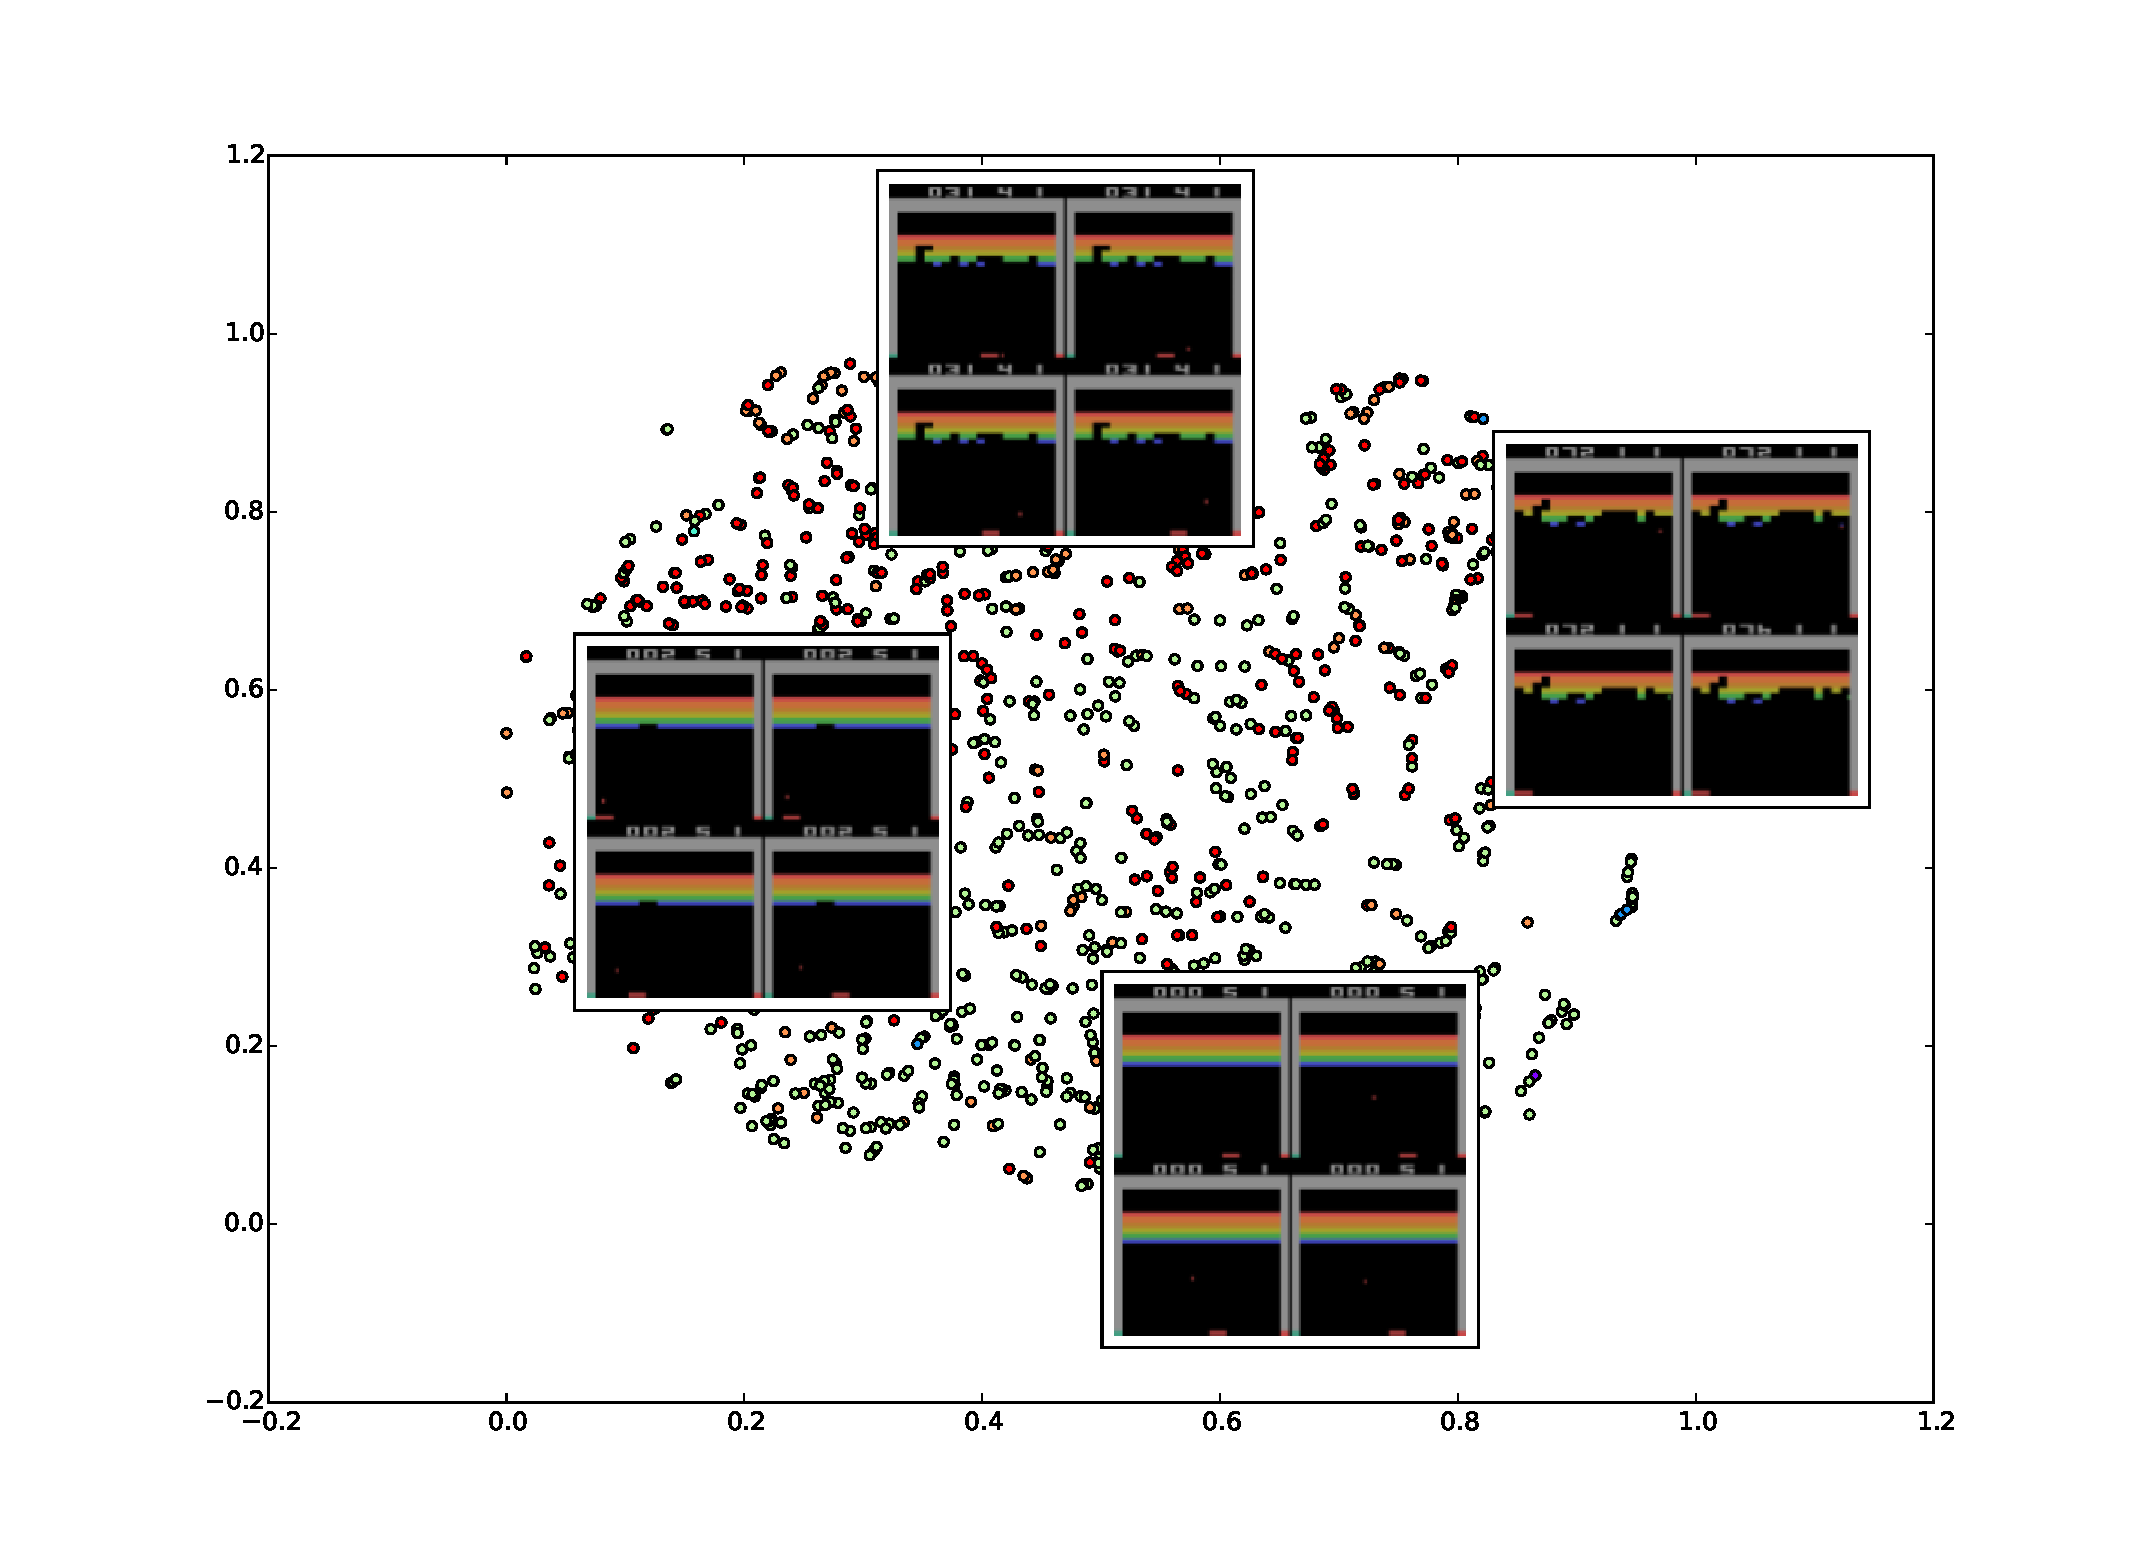
\includegraphics[width=1\textwidth]{../plots/tsne_breakout_new3_big.pdf}

\end{frame}
\section{Background}
\subsection{Computer Chess}
\begin{frame}{Background}{Computer Chess}
Shannon described the following ideal evaluation function.
\stepcounter{beamerpauses}
\begin{itemize}[<+->]
 \item Assign all the positions with no further play possible as:
\[f(position) = \begin{cases}
1 \text{ , if White has won}\\
0 \text{ , if it is a draw}\\
-1 \text{ , if Black has won}
\end{cases}\]
Use the recursive rule up the game tree:
\[f(p) = \max\limits_{p\rightarrow p'} (-f(p'))\]
where $p'$ is a position reachable in one move from position $p$.
\item Since, it is infeasible to compute such an evaluation function, we rely on approximations of $f$ to evaluate a board position. Most of such evaluation functions have a strong component of material weights in it.
\end{itemize}
\end{frame}

\begin{frame}{Background}{Computers playing chess}
\label{subsection:conventional-chess}
The fundamental implementation details of chess-playing computer system include:
\uncover<2->{
\begin{itemize}
\item \textbf{Board Representation} -- how a board position is represented in a 
data structure. The performance of move generation and piece evaluation depends 
on the data structure used to represent the board position.
\item \textbf{Search Techniques} -- how to identify and select the moves for 
further evaluation. Some of the most widely used search techniques are-- 
Minmax, Negamax, Negascout, Iterative deepening depth-first search etc. 
\item\textbf{Leaf Evaluation} -- how to evaluate the position of the board if 
no further evaluation needs to be done.
\end{itemize}
}
\end{frame}

\subsection{Deep Learning}
\begin{frame}{Background}{Deep Learning}
\begin{figure}[H]
\begin{tikzpicture}[
init/.style={
  draw,
  circle,
  inner sep=2pt,
  font=\Huge,
  join = by -latex
},
squa/.style={
  draw,
  inner sep=2pt,
  font=\Large,
  join = by -latex
},
start chain=2,node distance=13mm
]
\node[on chain=2] 
  (x2) {$x_2$};
\node[on chain=2,join=by o-latex] 
  {$w_2$};
\node[on chain=2,init] (sigma) 
  {$\displaystyle\Sigma$};
\node[on chain=2,squa,label=above:{\parbox{2cm}{\centering Activate \\ 
function}}]   
  {$f$};
\node[on chain=2,label=above:Output,join=by -latex] 
  {$y$};
\begin{scope}[start chain=1]
\node[on chain=1] at (0,1.5cm) 
  (x1) {$x_1$};
\node[on chain=1,join=by o-latex] 
  (w1) {$w_1$};
\end{scope}
\begin{scope}[start chain=3]
\node[on chain=3] at (0,-1.5cm) 
  (x3) {$x_3$};
\node[on chain=3,label=below:Weights,join=by o-latex] 
  (w3) {$w_3$};
\end{scope}
\node[label=above:\parbox{2cm}{\centering Bias \\ $b$}] at (sigma|-w1) (b) {};

\draw[-latex] (w1) -- (sigma);
\draw[-latex] (w3) -- (sigma);
\draw[o-latex] (b) -- (sigma);

\draw[decorate,decoration={brace,mirror}] (x1.north west) -- node[left=10pt] 
{Inputs} (x3.south west);
\end{tikzpicture}
\caption{An artificial neuron as a mathematical model}
\end{figure}
An artificial neuron inspire by a biological neuron is the basic component of an artificial neural network.\\
It computes $f(\sum_i w_ix_i + b)$, where $f$ is the activation function, $w_i$ is the weight given to the input from one of its dendrites.
\end{frame}

\begin{frame}{Background}{Artificial Neural Network}
 A combination of such neurons makes up an artificial neural network.
 \begin{figure}[H]
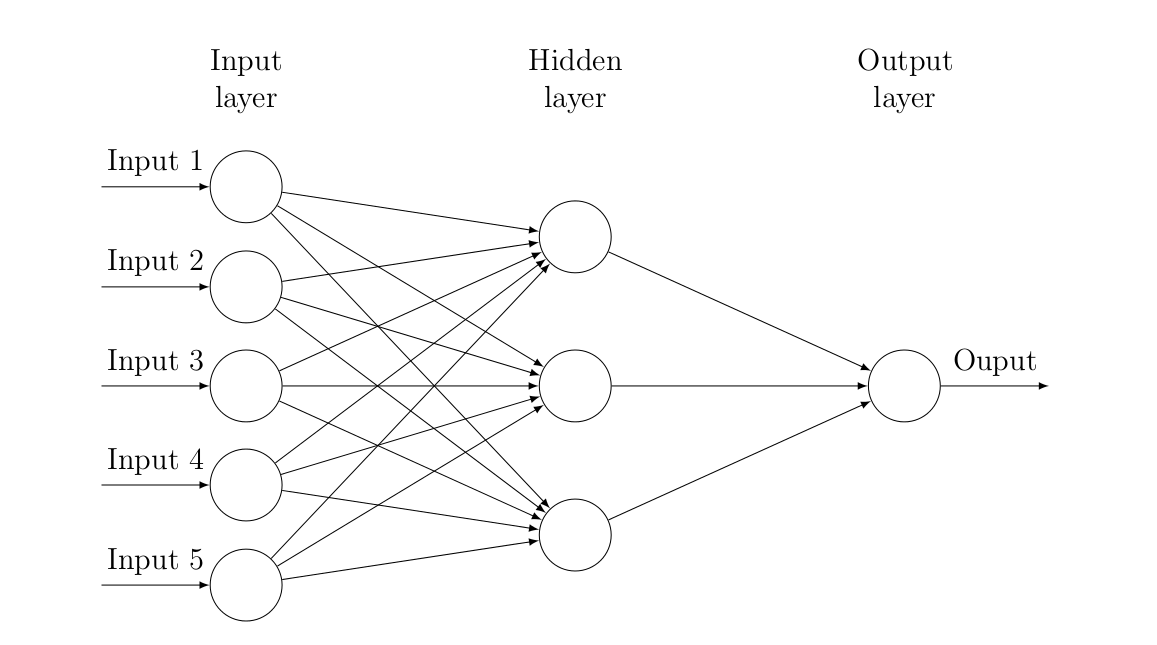
\includegraphics[width=0.9\textwidth]{../img/ann.png}
\caption{A two layer Artificial Neural network}
\end{figure}
\end{frame}

\begin{frame}{Background}{Universal Approximation Properties of Multilayer Perceptrons}
\begin{itemize}
 \item Hornick (1989) proved that 
Neural networks with at least one hidden layer are universal 
approximators.
\item This means that given any continuous 
function $f(x)$ and some $\epsilon>0$, a Neural network with one hidden layer 
containing a sufficient number of hidden layer neurons and a suitable choice of 
non-linearity, say represented by $g(x)$, exists such that $\forall x, 
|f(x)-g(x)|<\epsilon$.
\item In other words, we can approximate any given real 
valued continuous function with a two layer Neural network upto a certain 
accuracy.
\item The fact that two layer Neural networks are universal approximators 
is a pretty useless property in the case of machine learning. Neither does it 
tell the number of hidden units required to represent a given function upto the 
desired precision, nor does it promise that it represents a generalized 
function that fits the unseen data. 
\item The generalized function is expected to be smooth, 
while the overly precise two-layer network may overfit for the input data and 
not learn a promising representation.
\end{itemize}
\end{frame}

\subsection{Convolutional Neural Networks}
\begin{frame}[shrink=10]{Background}{Convolutional Neural Networks}
  Convolutional neural 
networks are nothing but neural networks which use convolution instead of 
full matrix multiplications in atleast one of the layers (Bengio, 2015).
\begin{figure}[H]
\centering
\begin{tikzpicture}

				\node at (0.5,-0.75){\begin{tabular}{c}input 
image\end{tabular}};
		
				\draw (0,0) -- (1,0) -- (1,1) -- (0,1) -- (0,0);
		
				\node at 
(3,3.25){\begin{tabular}{c}convolutional layer\\with 
non-linearities\end{tabular}};
		
				\draw[fill=black,opacity=0.2,draw=black] 
(2.75,1.25) -- (3.75,1.25) -- (3.75,2.25) -- (2.75,2.25) -- (2.75,1.25);
				\draw[fill=black,opacity=0.2,draw=black] 
(2.5,1) 
-- (3.5,1) -- (3.5,2) -- (2.5,2) -- (2.5,1);
				\draw[fill=black,opacity=0.2,draw=black] 
(2.25,0.75) -- (3.25,0.75) -- (3.25,1.75) -- (2.25,1.75) -- (2.25,0.75);
				\draw[fill=black,opacity=0.2,draw=black] 
(2,0.5) 
-- (3,0.5) -- (3,1.5) -- (2,1.5) -- (2,0.5);
				\draw[fill=black,opacity=0.2,draw=black] 
(1.75,0.25) -- (2.75,0.25) -- (2.75,1.25) -- (1.75,1.25) -- (1.75,0.25);
				\draw[fill=black,opacity=0.2,draw=black] 
(1.5,0) 
-- (2.5,0) -- (2.5,1) -- (1.5,1) -- (1.5,0);
		
				\node at 
(4.5,-0.75){\begin{tabular}{c}subsampling layer\end{tabular}};
		
				\draw[fill=black,opacity=0.2,draw=black] 
(5,1.25) -- (5.75,1.25) -- (5.75,2) -- (5,2) -- (5,1.25);
				\draw[fill=black,opacity=0.2,draw=black] 
(4.75,1) -- (5.5,1) -- (5.5,1.75) -- (4.75,1.75) -- (4.75,1);
				\draw[fill=black,opacity=0.2,draw=black] 
(4.5,0.75) -- (5.25,0.75) -- (5.25,1.5) -- (4.5,1.5) -- (4.5,0.75);
				\draw[fill=black,opacity=0.2,draw=black] 
(4.25,0.5) -- (5,0.5) -- (5,1.25) -- (4.25,1.25) -- (4.25,0.5);
				\draw[fill=black,opacity=0.2,draw=black] 
(4,0.25) -- (4.75,0.25) -- (4.75,1) -- (4,1) -- (4,0.25);
				\draw[fill=black,opacity=0.2,draw=black] 
(3.75,0) -- (4.5,0) -- (4.5,0.75) -- (3.75,0.75) -- (3.75,0);
		
% %				\node at 
% (7,3.5){\begin{tabular}{c}convolutional 
% layer\\with non-linearities\\layer $l = 4$\end{tabular}};
% %		
% %				\draw[fill=black,opacity=0.2,draw=black] 
% (7.5,1.75) -- (8.25,1.75) -- (8.25,2.5) -- (7.5,2.5) -- (7.5,1.75);
% %				\draw[fill=black,opacity=0.2,draw=black] 
% (7.25,1.5) -- (8,1.5) -- (8,2.25) -- (7.25,2.25) -- (7.25,1.5);
% %				\draw[fill=black,opacity=0.2,draw=black] 
% (7,1.25) -- (7.75,1.25) -- (7.75,2) -- (7,2) -- (7,1.25);
% %				\draw[fill=black,opacity=0.2,draw=black] 
% (6.75,1) -- (7.5,1) -- (7.5,1.75) -- (6.75,1.75) -- (6.75,1);
% %				\draw[fill=black,opacity=0.2,draw=black] 
% (6.5,0.75) -- (7.25,0.75) -- (7.25,1.5) -- (6.5,1.5) -- (6.5,0.75);
% %				\draw[fill=black,opacity=0.2,draw=black] 
% (6.25,0.5) -- (7,0.5) -- (7,1.25) -- (6.25,1.25) -- (6.25,0.5);
% %				\draw[fill=black,opacity=0.2,draw=black] 
% (6,0.25) -- (6.75,0.25) -- (6.75,1) -- (6,1) -- (6,0.25);
% %				\draw[fill=black,opacity=0.2,draw=black] 
% (5.75,0) -- (6.5,0) -- (6.5,0.75) -- (5.75,0.75) -- (5.75,0);
% %		
% %				\node at (9.5,-1){\begin{tabular}{c}subsampling 
% layer\\layer $l = 6$\end{tabular}};
% 		
% %				\draw[fill=black,opacity=0.2,draw=black] 
% (10,1.75) -- (10.5,1.75) -- (10.5,2.25) -- (10,2.25) -- (10,1.75);
% %				\draw[fill=black,opacity=0.2,draw=black] 
% (9.75,1.5) -- (10.25,1.5) -- (10.25,2) -- (9.75,2) -- (9.75,1.5);
% %				\draw[fill=black,opacity=0.2,draw=black] 
% (9.5,1.25) -- (10,1.25) -- (10,1.75) -- (9.5,1.75) -- (9.5,1.25);
% %				\draw[fill=black,opacity=0.2,draw=black] 
% (9.25,1) -- (9.75,1) -- (9.75,1.5) -- (9.25,1.5) -- (9.25,1);
% %				\draw[fill=black,opacity=0.2,draw=black] 
% (9,0.75) -- (9.5,0.75) -- (9.5,1.25) -- (9,1.25) -- (9,0.75);
% %				\draw[fill=black,opacity=0.2,draw=black] 
% (8.75,0.5) -- (9.25,0.5) -- (9.25,1) -- (8.75,1) -- (8.75,0.5);
% %				\draw[fill=black,opacity=0.2,draw=black] 
% (8.5,0.25) -- (9,0.25) -- (9,0.75) -- (8.5,0.75) -- (8.5,0.25);
% %				\draw[fill=black,opacity=0.2,draw=black] 
% (8.25,0) -- (8.75,0) -- (8.75,0.5) -- (8.25,0.5) -- (8.25,0);
% 		
				\node at (6.5,1){$\ldots$};
		
				\node at (8.5,3.25){\begin{tabular}{c}two-layer 
perceptron\end{tabular}};
		
				\draw[fill=black,draw=black,opacity=0.5] 
(6.5,0) 
-- (7,0) -- (8.5,1.75) -- (8,1.75) -- (6.5,0);
		
% 				%\node at (9,-1){\begin{tabular}{c}fully 
% connected layer\\output layer $l = 8$\end{tabular}};
		
				\draw[fill=black,draw=black,opacity=0.5] 
(8.5,0.5) -- (9,0.5) -- (9.65,1.25) -- (9.15,1.25) -- (8.5,0.5);
\end{tikzpicture}
\caption{A typical Convolutional Neural Network architecture}			
\end{figure}
It is the most successful approach for almost all recognition and
detection tasks in computer vision (Krizhevsky et al., 2012; Tompson et al., 2014;
Taigman et al., 2014) and even approaches human performance on some tasks
(Ciresan et al., 2012)
\end{frame}

\section{Dataset}
\begin{frame}{Dataset}{Acquisition}
\begin{table}[H]
\tiny\centering
\begin{tabular}{@{}lll@{}}
\toprule
Dataset Name & Number of Games 	& Total number of boards  \\
\midrule
CvC 2009-14  & $370,480$	& $74,162,875$             \\ 
FICS 2014 (avg ELO$>$2000)    & $522,356$    	& $32,598,059$      \\
FICS 2014 (all ELO, subset) & $\sim 1M$ & $\sim 125M$\\
\bottomrule
\end{tabular}
\end{table}

\begin{figure}
  \hspace{0.5in}
  \scalebox{.4}{%% Creator: Matplotlib, PGF backend
%%
%% To include the figure in your LaTeX document, write
%%   \input{<filename>.pgf}
%%
%% Make sure the required packages are loaded in your preamble
%%   \usepackage{pgf}
%%
%% Figures using additional raster images can only be included by \input if
%% they are in the same directory as the main LaTeX file. For loading figures
%% from other directories you can use the `import` package
%%   \usepackage{import}
%% and then include the figures with
%%   \import{<path to file>}{<filename>.pgf}
%%
%% Matplotlib used the following preamble
%%   \usepackage{fontspec}
%%   \setmainfont{DejaVu Serif}
%%   \setsansfont{DejaVu Sans}
%%   \setmonofont{DejaVu Sans Mono}
%%
\begingroup%
\makeatletter%
\begin{pgfpicture}%
\pgfpathrectangle{\pgfpointorigin}{\pgfqpoint{8.000000in}{6.000000in}}%
\pgfusepath{use as bounding box, clip}%
\begin{pgfscope}%
\pgfsetbuttcap%
\pgfsetmiterjoin%
\definecolor{currentfill}{rgb}{1.000000,1.000000,1.000000}%
\pgfsetfillcolor{currentfill}%
\pgfsetlinewidth{0.000000pt}%
\definecolor{currentstroke}{rgb}{1.000000,1.000000,1.000000}%
\pgfsetstrokecolor{currentstroke}%
\pgfsetdash{}{0pt}%
\pgfpathmoveto{\pgfqpoint{0.000000in}{0.000000in}}%
\pgfpathlineto{\pgfqpoint{8.000000in}{0.000000in}}%
\pgfpathlineto{\pgfqpoint{8.000000in}{6.000000in}}%
\pgfpathlineto{\pgfqpoint{0.000000in}{6.000000in}}%
\pgfpathclose%
\pgfusepath{fill}%
\end{pgfscope}%
\begin{pgfscope}%
\pgfsetbuttcap%
\pgfsetmiterjoin%
\definecolor{currentfill}{rgb}{1.000000,1.000000,1.000000}%
\pgfsetfillcolor{currentfill}%
\pgfsetlinewidth{0.000000pt}%
\definecolor{currentstroke}{rgb}{0.000000,0.000000,0.000000}%
\pgfsetstrokecolor{currentstroke}%
\pgfsetstrokeopacity{0.000000}%
\pgfsetdash{}{0pt}%
\pgfpathmoveto{\pgfqpoint{1.000000in}{0.600000in}}%
\pgfpathlineto{\pgfqpoint{7.200000in}{0.600000in}}%
\pgfpathlineto{\pgfqpoint{7.200000in}{5.400000in}}%
\pgfpathlineto{\pgfqpoint{1.000000in}{5.400000in}}%
\pgfpathclose%
\pgfusepath{fill}%
\end{pgfscope}%
\begin{pgfscope}%
\pgfpathrectangle{\pgfqpoint{1.000000in}{0.600000in}}{\pgfqpoint{6.200000in}{4.800000in}} %
\pgfusepath{clip}%
\pgfsetbuttcap%
\pgfsetmiterjoin%
\definecolor{currentfill}{rgb}{0.827451,0.827451,0.827451}%
\pgfsetfillcolor{currentfill}%
\pgfsetlinewidth{1.003750pt}%
\definecolor{currentstroke}{rgb}{0.000000,0.000000,0.000000}%
\pgfsetstrokecolor{currentstroke}%
\pgfsetdash{}{0pt}%
\pgfpathmoveto{\pgfqpoint{1.000000in}{0.600000in}}%
\pgfpathlineto{\pgfqpoint{1.258333in}{0.600000in}}%
\pgfpathlineto{\pgfqpoint{1.258333in}{5.180894in}}%
\pgfpathlineto{\pgfqpoint{1.000000in}{5.180894in}}%
\pgfpathlineto{\pgfqpoint{1.000000in}{0.600000in}}%
\pgfusepath{stroke,fill}%
\end{pgfscope}%
\begin{pgfscope}%
\pgfpathrectangle{\pgfqpoint{1.000000in}{0.600000in}}{\pgfqpoint{6.200000in}{4.800000in}} %
\pgfusepath{clip}%
\pgfsetbuttcap%
\pgfsetmiterjoin%
\definecolor{currentfill}{rgb}{0.827451,0.827451,0.827451}%
\pgfsetfillcolor{currentfill}%
\pgfsetlinewidth{1.003750pt}%
\definecolor{currentstroke}{rgb}{0.000000,0.000000,0.000000}%
\pgfsetstrokecolor{currentstroke}%
\pgfsetdash{}{0pt}%
\pgfpathmoveto{\pgfqpoint{2.033333in}{0.600000in}}%
\pgfpathlineto{\pgfqpoint{2.291667in}{0.600000in}}%
\pgfpathlineto{\pgfqpoint{2.291667in}{3.479202in}}%
\pgfpathlineto{\pgfqpoint{2.033333in}{3.479202in}}%
\pgfpathlineto{\pgfqpoint{2.033333in}{0.600000in}}%
\pgfusepath{stroke,fill}%
\end{pgfscope}%
\begin{pgfscope}%
\pgfpathrectangle{\pgfqpoint{1.000000in}{0.600000in}}{\pgfqpoint{6.200000in}{4.800000in}} %
\pgfusepath{clip}%
\pgfsetbuttcap%
\pgfsetmiterjoin%
\definecolor{currentfill}{rgb}{0.827451,0.827451,0.827451}%
\pgfsetfillcolor{currentfill}%
\pgfsetlinewidth{1.003750pt}%
\definecolor{currentstroke}{rgb}{0.000000,0.000000,0.000000}%
\pgfsetstrokecolor{currentstroke}%
\pgfsetdash{}{0pt}%
\pgfpathmoveto{\pgfqpoint{3.066667in}{0.600000in}}%
\pgfpathlineto{\pgfqpoint{3.325000in}{0.600000in}}%
\pgfpathlineto{\pgfqpoint{3.325000in}{3.442842in}}%
\pgfpathlineto{\pgfqpoint{3.066667in}{3.442842in}}%
\pgfpathlineto{\pgfqpoint{3.066667in}{0.600000in}}%
\pgfusepath{stroke,fill}%
\end{pgfscope}%
\begin{pgfscope}%
\pgfpathrectangle{\pgfqpoint{1.000000in}{0.600000in}}{\pgfqpoint{6.200000in}{4.800000in}} %
\pgfusepath{clip}%
\pgfsetbuttcap%
\pgfsetmiterjoin%
\definecolor{currentfill}{rgb}{0.827451,0.827451,0.827451}%
\pgfsetfillcolor{currentfill}%
\pgfsetlinewidth{1.003750pt}%
\definecolor{currentstroke}{rgb}{0.000000,0.000000,0.000000}%
\pgfsetstrokecolor{currentstroke}%
\pgfsetdash{}{0pt}%
\pgfpathmoveto{\pgfqpoint{4.100000in}{0.600000in}}%
\pgfpathlineto{\pgfqpoint{4.358333in}{0.600000in}}%
\pgfpathlineto{\pgfqpoint{4.358333in}{3.232154in}}%
\pgfpathlineto{\pgfqpoint{4.100000in}{3.232154in}}%
\pgfpathlineto{\pgfqpoint{4.100000in}{0.600000in}}%
\pgfusepath{stroke,fill}%
\end{pgfscope}%
\begin{pgfscope}%
\pgfpathrectangle{\pgfqpoint{1.000000in}{0.600000in}}{\pgfqpoint{6.200000in}{4.800000in}} %
\pgfusepath{clip}%
\pgfsetbuttcap%
\pgfsetmiterjoin%
\definecolor{currentfill}{rgb}{0.827451,0.827451,0.827451}%
\pgfsetfillcolor{currentfill}%
\pgfsetlinewidth{1.003750pt}%
\definecolor{currentstroke}{rgb}{0.000000,0.000000,0.000000}%
\pgfsetstrokecolor{currentstroke}%
\pgfsetdash{}{0pt}%
\pgfpathmoveto{\pgfqpoint{5.133333in}{0.600000in}}%
\pgfpathlineto{\pgfqpoint{5.391667in}{0.600000in}}%
\pgfpathlineto{\pgfqpoint{5.391667in}{2.688066in}}%
\pgfpathlineto{\pgfqpoint{5.133333in}{2.688066in}}%
\pgfpathlineto{\pgfqpoint{5.133333in}{0.600000in}}%
\pgfusepath{stroke,fill}%
\end{pgfscope}%
\begin{pgfscope}%
\pgfpathrectangle{\pgfqpoint{1.000000in}{0.600000in}}{\pgfqpoint{6.200000in}{4.800000in}} %
\pgfusepath{clip}%
\pgfsetbuttcap%
\pgfsetmiterjoin%
\definecolor{currentfill}{rgb}{0.827451,0.827451,0.827451}%
\pgfsetfillcolor{currentfill}%
\pgfsetlinewidth{1.003750pt}%
\definecolor{currentstroke}{rgb}{0.000000,0.000000,0.000000}%
\pgfsetstrokecolor{currentstroke}%
\pgfsetdash{}{0pt}%
\pgfpathmoveto{\pgfqpoint{6.166667in}{0.600000in}}%
\pgfpathlineto{\pgfqpoint{6.425000in}{0.600000in}}%
\pgfpathlineto{\pgfqpoint{6.425000in}{2.962474in}}%
\pgfpathlineto{\pgfqpoint{6.166667in}{2.962474in}}%
\pgfpathlineto{\pgfqpoint{6.166667in}{0.600000in}}%
\pgfusepath{stroke,fill}%
\end{pgfscope}%
\begin{pgfscope}%
\pgfpathrectangle{\pgfqpoint{1.000000in}{0.600000in}}{\pgfqpoint{6.200000in}{4.800000in}} %
\pgfusepath{clip}%
\pgfsetbuttcap%
\pgfsetmiterjoin%
\definecolor{currentfill}{rgb}{0.117647,0.564706,1.000000}%
\pgfsetfillcolor{currentfill}%
\pgfsetlinewidth{1.003750pt}%
\definecolor{currentstroke}{rgb}{0.000000,0.000000,0.000000}%
\pgfsetstrokecolor{currentstroke}%
\pgfsetdash{}{0pt}%
\pgfpathmoveto{\pgfqpoint{1.258333in}{0.600000in}}%
\pgfpathlineto{\pgfqpoint{1.516667in}{0.600000in}}%
\pgfpathlineto{\pgfqpoint{1.516667in}{5.381416in}}%
\pgfpathlineto{\pgfqpoint{1.258333in}{5.381416in}}%
\pgfpathlineto{\pgfqpoint{1.258333in}{0.600000in}}%
\pgfusepath{stroke,fill}%
\end{pgfscope}%
\begin{pgfscope}%
\pgfpathrectangle{\pgfqpoint{1.000000in}{0.600000in}}{\pgfqpoint{6.200000in}{4.800000in}} %
\pgfusepath{clip}%
\pgfsetbuttcap%
\pgfsetmiterjoin%
\definecolor{currentfill}{rgb}{0.117647,0.564706,1.000000}%
\pgfsetfillcolor{currentfill}%
\pgfsetlinewidth{1.003750pt}%
\definecolor{currentstroke}{rgb}{0.000000,0.000000,0.000000}%
\pgfsetstrokecolor{currentstroke}%
\pgfsetdash{}{0pt}%
\pgfpathmoveto{\pgfqpoint{2.291667in}{0.600000in}}%
\pgfpathlineto{\pgfqpoint{2.550000in}{0.600000in}}%
\pgfpathlineto{\pgfqpoint{2.550000in}{5.009714in}}%
\pgfpathlineto{\pgfqpoint{2.291667in}{5.009714in}}%
\pgfpathlineto{\pgfqpoint{2.291667in}{0.600000in}}%
\pgfusepath{stroke,fill}%
\end{pgfscope}%
\begin{pgfscope}%
\pgfpathrectangle{\pgfqpoint{1.000000in}{0.600000in}}{\pgfqpoint{6.200000in}{4.800000in}} %
\pgfusepath{clip}%
\pgfsetbuttcap%
\pgfsetmiterjoin%
\definecolor{currentfill}{rgb}{0.117647,0.564706,1.000000}%
\pgfsetfillcolor{currentfill}%
\pgfsetlinewidth{1.003750pt}%
\definecolor{currentstroke}{rgb}{0.000000,0.000000,0.000000}%
\pgfsetstrokecolor{currentstroke}%
\pgfsetdash{}{0pt}%
\pgfpathmoveto{\pgfqpoint{3.325000in}{0.600000in}}%
\pgfpathlineto{\pgfqpoint{3.583333in}{0.600000in}}%
\pgfpathlineto{\pgfqpoint{3.583333in}{3.555010in}}%
\pgfpathlineto{\pgfqpoint{3.325000in}{3.555010in}}%
\pgfpathlineto{\pgfqpoint{3.325000in}{0.600000in}}%
\pgfusepath{stroke,fill}%
\end{pgfscope}%
\begin{pgfscope}%
\pgfpathrectangle{\pgfqpoint{1.000000in}{0.600000in}}{\pgfqpoint{6.200000in}{4.800000in}} %
\pgfusepath{clip}%
\pgfsetbuttcap%
\pgfsetmiterjoin%
\definecolor{currentfill}{rgb}{0.117647,0.564706,1.000000}%
\pgfsetfillcolor{currentfill}%
\pgfsetlinewidth{1.003750pt}%
\definecolor{currentstroke}{rgb}{0.000000,0.000000,0.000000}%
\pgfsetstrokecolor{currentstroke}%
\pgfsetdash{}{0pt}%
\pgfpathmoveto{\pgfqpoint{4.358333in}{0.600000in}}%
\pgfpathlineto{\pgfqpoint{4.616667in}{0.600000in}}%
\pgfpathlineto{\pgfqpoint{4.616667in}{3.841903in}}%
\pgfpathlineto{\pgfqpoint{4.358333in}{3.841903in}}%
\pgfpathlineto{\pgfqpoint{4.358333in}{0.600000in}}%
\pgfusepath{stroke,fill}%
\end{pgfscope}%
\begin{pgfscope}%
\pgfpathrectangle{\pgfqpoint{1.000000in}{0.600000in}}{\pgfqpoint{6.200000in}{4.800000in}} %
\pgfusepath{clip}%
\pgfsetbuttcap%
\pgfsetmiterjoin%
\definecolor{currentfill}{rgb}{0.117647,0.564706,1.000000}%
\pgfsetfillcolor{currentfill}%
\pgfsetlinewidth{1.003750pt}%
\definecolor{currentstroke}{rgb}{0.000000,0.000000,0.000000}%
\pgfsetstrokecolor{currentstroke}%
\pgfsetdash{}{0pt}%
\pgfpathmoveto{\pgfqpoint{5.391667in}{0.600000in}}%
\pgfpathlineto{\pgfqpoint{5.650000in}{0.600000in}}%
\pgfpathlineto{\pgfqpoint{5.650000in}{3.505016in}}%
\pgfpathlineto{\pgfqpoint{5.391667in}{3.505016in}}%
\pgfpathlineto{\pgfqpoint{5.391667in}{0.600000in}}%
\pgfusepath{stroke,fill}%
\end{pgfscope}%
\begin{pgfscope}%
\pgfpathrectangle{\pgfqpoint{1.000000in}{0.600000in}}{\pgfqpoint{6.200000in}{4.800000in}} %
\pgfusepath{clip}%
\pgfsetbuttcap%
\pgfsetmiterjoin%
\definecolor{currentfill}{rgb}{0.117647,0.564706,1.000000}%
\pgfsetfillcolor{currentfill}%
\pgfsetlinewidth{1.003750pt}%
\definecolor{currentstroke}{rgb}{0.000000,0.000000,0.000000}%
\pgfsetstrokecolor{currentstroke}%
\pgfsetdash{}{0pt}%
\pgfpathmoveto{\pgfqpoint{6.425000in}{0.600000in}}%
\pgfpathlineto{\pgfqpoint{6.683333in}{0.600000in}}%
\pgfpathlineto{\pgfqpoint{6.683333in}{4.474843in}}%
\pgfpathlineto{\pgfqpoint{6.425000in}{4.474843in}}%
\pgfpathlineto{\pgfqpoint{6.425000in}{0.600000in}}%
\pgfusepath{stroke,fill}%
\end{pgfscope}%
\begin{pgfscope}%
\pgfsetrectcap%
\pgfsetmiterjoin%
\pgfsetlinewidth{1.003750pt}%
\definecolor{currentstroke}{rgb}{0.000000,0.000000,0.000000}%
\pgfsetstrokecolor{currentstroke}%
\pgfsetdash{}{0pt}%
\pgfpathmoveto{\pgfqpoint{1.000000in}{5.400000in}}%
\pgfpathlineto{\pgfqpoint{7.200000in}{5.400000in}}%
\pgfusepath{stroke}%
\end{pgfscope}%
\begin{pgfscope}%
\pgfsetrectcap%
\pgfsetmiterjoin%
\pgfsetlinewidth{1.003750pt}%
\definecolor{currentstroke}{rgb}{0.000000,0.000000,0.000000}%
\pgfsetstrokecolor{currentstroke}%
\pgfsetdash{}{0pt}%
\pgfpathmoveto{\pgfqpoint{7.200000in}{0.600000in}}%
\pgfpathlineto{\pgfqpoint{7.200000in}{5.400000in}}%
\pgfusepath{stroke}%
\end{pgfscope}%
\begin{pgfscope}%
\pgfsetrectcap%
\pgfsetmiterjoin%
\pgfsetlinewidth{1.003750pt}%
\definecolor{currentstroke}{rgb}{0.000000,0.000000,0.000000}%
\pgfsetstrokecolor{currentstroke}%
\pgfsetdash{}{0pt}%
\pgfpathmoveto{\pgfqpoint{1.000000in}{0.600000in}}%
\pgfpathlineto{\pgfqpoint{7.200000in}{0.600000in}}%
\pgfusepath{stroke}%
\end{pgfscope}%
\begin{pgfscope}%
\pgfsetrectcap%
\pgfsetmiterjoin%
\pgfsetlinewidth{1.003750pt}%
\definecolor{currentstroke}{rgb}{0.000000,0.000000,0.000000}%
\pgfsetstrokecolor{currentstroke}%
\pgfsetdash{}{0pt}%
\pgfpathmoveto{\pgfqpoint{1.000000in}{0.600000in}}%
\pgfpathlineto{\pgfqpoint{1.000000in}{5.400000in}}%
\pgfusepath{stroke}%
\end{pgfscope}%
\begin{pgfscope}%
\pgfsetbuttcap%
\pgfsetroundjoin%
\definecolor{currentfill}{rgb}{0.000000,0.000000,0.000000}%
\pgfsetfillcolor{currentfill}%
\pgfsetlinewidth{0.501875pt}%
\definecolor{currentstroke}{rgb}{0.000000,0.000000,0.000000}%
\pgfsetstrokecolor{currentstroke}%
\pgfsetdash{}{0pt}%
\pgfsys@defobject{currentmarker}{\pgfqpoint{0.000000in}{0.000000in}}{\pgfqpoint{0.000000in}{0.055556in}}{%
\pgfpathmoveto{\pgfqpoint{0.000000in}{0.000000in}}%
\pgfpathlineto{\pgfqpoint{0.000000in}{0.055556in}}%
\pgfusepath{stroke,fill}%
}%
\begin{pgfscope}%
\pgfsys@transformshift{1.258333in}{0.600000in}%
\pgfsys@useobject{currentmarker}{}%
\end{pgfscope}%
\end{pgfscope}%
\begin{pgfscope}%
\pgfsetbuttcap%
\pgfsetroundjoin%
\definecolor{currentfill}{rgb}{0.000000,0.000000,0.000000}%
\pgfsetfillcolor{currentfill}%
\pgfsetlinewidth{0.501875pt}%
\definecolor{currentstroke}{rgb}{0.000000,0.000000,0.000000}%
\pgfsetstrokecolor{currentstroke}%
\pgfsetdash{}{0pt}%
\pgfsys@defobject{currentmarker}{\pgfqpoint{0.000000in}{-0.055556in}}{\pgfqpoint{0.000000in}{0.000000in}}{%
\pgfpathmoveto{\pgfqpoint{0.000000in}{0.000000in}}%
\pgfpathlineto{\pgfqpoint{0.000000in}{-0.055556in}}%
\pgfusepath{stroke,fill}%
}%
\begin{pgfscope}%
\pgfsys@transformshift{1.258333in}{5.400000in}%
\pgfsys@useobject{currentmarker}{}%
\end{pgfscope}%
\end{pgfscope}%
\begin{pgfscope}%
\pgftext[x=1.258333in,y=0.544444in,,top]{\rmfamily\fontsize{12.000000}{14.400000}\selectfont Pawn}%
\end{pgfscope}%
\begin{pgfscope}%
\pgfsetbuttcap%
\pgfsetroundjoin%
\definecolor{currentfill}{rgb}{0.000000,0.000000,0.000000}%
\pgfsetfillcolor{currentfill}%
\pgfsetlinewidth{0.501875pt}%
\definecolor{currentstroke}{rgb}{0.000000,0.000000,0.000000}%
\pgfsetstrokecolor{currentstroke}%
\pgfsetdash{}{0pt}%
\pgfsys@defobject{currentmarker}{\pgfqpoint{0.000000in}{0.000000in}}{\pgfqpoint{0.000000in}{0.055556in}}{%
\pgfpathmoveto{\pgfqpoint{0.000000in}{0.000000in}}%
\pgfpathlineto{\pgfqpoint{0.000000in}{0.055556in}}%
\pgfusepath{stroke,fill}%
}%
\begin{pgfscope}%
\pgfsys@transformshift{2.291667in}{0.600000in}%
\pgfsys@useobject{currentmarker}{}%
\end{pgfscope}%
\end{pgfscope}%
\begin{pgfscope}%
\pgfsetbuttcap%
\pgfsetroundjoin%
\definecolor{currentfill}{rgb}{0.000000,0.000000,0.000000}%
\pgfsetfillcolor{currentfill}%
\pgfsetlinewidth{0.501875pt}%
\definecolor{currentstroke}{rgb}{0.000000,0.000000,0.000000}%
\pgfsetstrokecolor{currentstroke}%
\pgfsetdash{}{0pt}%
\pgfsys@defobject{currentmarker}{\pgfqpoint{0.000000in}{-0.055556in}}{\pgfqpoint{0.000000in}{0.000000in}}{%
\pgfpathmoveto{\pgfqpoint{0.000000in}{0.000000in}}%
\pgfpathlineto{\pgfqpoint{0.000000in}{-0.055556in}}%
\pgfusepath{stroke,fill}%
}%
\begin{pgfscope}%
\pgfsys@transformshift{2.291667in}{5.400000in}%
\pgfsys@useobject{currentmarker}{}%
\end{pgfscope}%
\end{pgfscope}%
\begin{pgfscope}%
\pgftext[x=2.291667in,y=0.544444in,,top]{\rmfamily\fontsize{12.000000}{14.400000}\selectfont Rook}%
\end{pgfscope}%
\begin{pgfscope}%
\pgfsetbuttcap%
\pgfsetroundjoin%
\definecolor{currentfill}{rgb}{0.000000,0.000000,0.000000}%
\pgfsetfillcolor{currentfill}%
\pgfsetlinewidth{0.501875pt}%
\definecolor{currentstroke}{rgb}{0.000000,0.000000,0.000000}%
\pgfsetstrokecolor{currentstroke}%
\pgfsetdash{}{0pt}%
\pgfsys@defobject{currentmarker}{\pgfqpoint{0.000000in}{0.000000in}}{\pgfqpoint{0.000000in}{0.055556in}}{%
\pgfpathmoveto{\pgfqpoint{0.000000in}{0.000000in}}%
\pgfpathlineto{\pgfqpoint{0.000000in}{0.055556in}}%
\pgfusepath{stroke,fill}%
}%
\begin{pgfscope}%
\pgfsys@transformshift{3.325000in}{0.600000in}%
\pgfsys@useobject{currentmarker}{}%
\end{pgfscope}%
\end{pgfscope}%
\begin{pgfscope}%
\pgfsetbuttcap%
\pgfsetroundjoin%
\definecolor{currentfill}{rgb}{0.000000,0.000000,0.000000}%
\pgfsetfillcolor{currentfill}%
\pgfsetlinewidth{0.501875pt}%
\definecolor{currentstroke}{rgb}{0.000000,0.000000,0.000000}%
\pgfsetstrokecolor{currentstroke}%
\pgfsetdash{}{0pt}%
\pgfsys@defobject{currentmarker}{\pgfqpoint{0.000000in}{-0.055556in}}{\pgfqpoint{0.000000in}{0.000000in}}{%
\pgfpathmoveto{\pgfqpoint{0.000000in}{0.000000in}}%
\pgfpathlineto{\pgfqpoint{0.000000in}{-0.055556in}}%
\pgfusepath{stroke,fill}%
}%
\begin{pgfscope}%
\pgfsys@transformshift{3.325000in}{5.400000in}%
\pgfsys@useobject{currentmarker}{}%
\end{pgfscope}%
\end{pgfscope}%
\begin{pgfscope}%
\pgftext[x=3.325000in,y=0.544444in,,top]{\rmfamily\fontsize{12.000000}{14.400000}\selectfont Knight}%
\end{pgfscope}%
\begin{pgfscope}%
\pgfsetbuttcap%
\pgfsetroundjoin%
\definecolor{currentfill}{rgb}{0.000000,0.000000,0.000000}%
\pgfsetfillcolor{currentfill}%
\pgfsetlinewidth{0.501875pt}%
\definecolor{currentstroke}{rgb}{0.000000,0.000000,0.000000}%
\pgfsetstrokecolor{currentstroke}%
\pgfsetdash{}{0pt}%
\pgfsys@defobject{currentmarker}{\pgfqpoint{0.000000in}{0.000000in}}{\pgfqpoint{0.000000in}{0.055556in}}{%
\pgfpathmoveto{\pgfqpoint{0.000000in}{0.000000in}}%
\pgfpathlineto{\pgfqpoint{0.000000in}{0.055556in}}%
\pgfusepath{stroke,fill}%
}%
\begin{pgfscope}%
\pgfsys@transformshift{4.358333in}{0.600000in}%
\pgfsys@useobject{currentmarker}{}%
\end{pgfscope}%
\end{pgfscope}%
\begin{pgfscope}%
\pgfsetbuttcap%
\pgfsetroundjoin%
\definecolor{currentfill}{rgb}{0.000000,0.000000,0.000000}%
\pgfsetfillcolor{currentfill}%
\pgfsetlinewidth{0.501875pt}%
\definecolor{currentstroke}{rgb}{0.000000,0.000000,0.000000}%
\pgfsetstrokecolor{currentstroke}%
\pgfsetdash{}{0pt}%
\pgfsys@defobject{currentmarker}{\pgfqpoint{0.000000in}{-0.055556in}}{\pgfqpoint{0.000000in}{0.000000in}}{%
\pgfpathmoveto{\pgfqpoint{0.000000in}{0.000000in}}%
\pgfpathlineto{\pgfqpoint{0.000000in}{-0.055556in}}%
\pgfusepath{stroke,fill}%
}%
\begin{pgfscope}%
\pgfsys@transformshift{4.358333in}{5.400000in}%
\pgfsys@useobject{currentmarker}{}%
\end{pgfscope}%
\end{pgfscope}%
\begin{pgfscope}%
\pgftext[x=4.358333in,y=0.544444in,,top]{\rmfamily\fontsize{12.000000}{14.400000}\selectfont Bishop}%
\end{pgfscope}%
\begin{pgfscope}%
\pgfsetbuttcap%
\pgfsetroundjoin%
\definecolor{currentfill}{rgb}{0.000000,0.000000,0.000000}%
\pgfsetfillcolor{currentfill}%
\pgfsetlinewidth{0.501875pt}%
\definecolor{currentstroke}{rgb}{0.000000,0.000000,0.000000}%
\pgfsetstrokecolor{currentstroke}%
\pgfsetdash{}{0pt}%
\pgfsys@defobject{currentmarker}{\pgfqpoint{0.000000in}{0.000000in}}{\pgfqpoint{0.000000in}{0.055556in}}{%
\pgfpathmoveto{\pgfqpoint{0.000000in}{0.000000in}}%
\pgfpathlineto{\pgfqpoint{0.000000in}{0.055556in}}%
\pgfusepath{stroke,fill}%
}%
\begin{pgfscope}%
\pgfsys@transformshift{5.391667in}{0.600000in}%
\pgfsys@useobject{currentmarker}{}%
\end{pgfscope}%
\end{pgfscope}%
\begin{pgfscope}%
\pgfsetbuttcap%
\pgfsetroundjoin%
\definecolor{currentfill}{rgb}{0.000000,0.000000,0.000000}%
\pgfsetfillcolor{currentfill}%
\pgfsetlinewidth{0.501875pt}%
\definecolor{currentstroke}{rgb}{0.000000,0.000000,0.000000}%
\pgfsetstrokecolor{currentstroke}%
\pgfsetdash{}{0pt}%
\pgfsys@defobject{currentmarker}{\pgfqpoint{0.000000in}{-0.055556in}}{\pgfqpoint{0.000000in}{0.000000in}}{%
\pgfpathmoveto{\pgfqpoint{0.000000in}{0.000000in}}%
\pgfpathlineto{\pgfqpoint{0.000000in}{-0.055556in}}%
\pgfusepath{stroke,fill}%
}%
\begin{pgfscope}%
\pgfsys@transformshift{5.391667in}{5.400000in}%
\pgfsys@useobject{currentmarker}{}%
\end{pgfscope}%
\end{pgfscope}%
\begin{pgfscope}%
\pgftext[x=5.391667in,y=0.544444in,,top]{\rmfamily\fontsize{12.000000}{14.400000}\selectfont Queen}%
\end{pgfscope}%
\begin{pgfscope}%
\pgfsetbuttcap%
\pgfsetroundjoin%
\definecolor{currentfill}{rgb}{0.000000,0.000000,0.000000}%
\pgfsetfillcolor{currentfill}%
\pgfsetlinewidth{0.501875pt}%
\definecolor{currentstroke}{rgb}{0.000000,0.000000,0.000000}%
\pgfsetstrokecolor{currentstroke}%
\pgfsetdash{}{0pt}%
\pgfsys@defobject{currentmarker}{\pgfqpoint{0.000000in}{0.000000in}}{\pgfqpoint{0.000000in}{0.055556in}}{%
\pgfpathmoveto{\pgfqpoint{0.000000in}{0.000000in}}%
\pgfpathlineto{\pgfqpoint{0.000000in}{0.055556in}}%
\pgfusepath{stroke,fill}%
}%
\begin{pgfscope}%
\pgfsys@transformshift{6.425000in}{0.600000in}%
\pgfsys@useobject{currentmarker}{}%
\end{pgfscope}%
\end{pgfscope}%
\begin{pgfscope}%
\pgfsetbuttcap%
\pgfsetroundjoin%
\definecolor{currentfill}{rgb}{0.000000,0.000000,0.000000}%
\pgfsetfillcolor{currentfill}%
\pgfsetlinewidth{0.501875pt}%
\definecolor{currentstroke}{rgb}{0.000000,0.000000,0.000000}%
\pgfsetstrokecolor{currentstroke}%
\pgfsetdash{}{0pt}%
\pgfsys@defobject{currentmarker}{\pgfqpoint{0.000000in}{-0.055556in}}{\pgfqpoint{0.000000in}{0.000000in}}{%
\pgfpathmoveto{\pgfqpoint{0.000000in}{0.000000in}}%
\pgfpathlineto{\pgfqpoint{0.000000in}{-0.055556in}}%
\pgfusepath{stroke,fill}%
}%
\begin{pgfscope}%
\pgfsys@transformshift{6.425000in}{5.400000in}%
\pgfsys@useobject{currentmarker}{}%
\end{pgfscope}%
\end{pgfscope}%
\begin{pgfscope}%
\pgftext[x=6.425000in,y=0.544444in,,top]{\rmfamily\fontsize{12.000000}{14.400000}\selectfont King}%
\end{pgfscope}%
\begin{pgfscope}%
\pgftext[x=4.100000in,y=0.311345in,,top]{\rmfamily\fontsize{12.000000}{14.400000}\selectfont Piece types}%
\end{pgfscope}%
\begin{pgfscope}%
\pgfsetbuttcap%
\pgfsetroundjoin%
\definecolor{currentfill}{rgb}{0.000000,0.000000,0.000000}%
\pgfsetfillcolor{currentfill}%
\pgfsetlinewidth{0.501875pt}%
\definecolor{currentstroke}{rgb}{0.000000,0.000000,0.000000}%
\pgfsetstrokecolor{currentstroke}%
\pgfsetdash{}{0pt}%
\pgfsys@defobject{currentmarker}{\pgfqpoint{0.000000in}{0.000000in}}{\pgfqpoint{0.055556in}{0.000000in}}{%
\pgfpathmoveto{\pgfqpoint{0.000000in}{0.000000in}}%
\pgfpathlineto{\pgfqpoint{0.055556in}{0.000000in}}%
\pgfusepath{stroke,fill}%
}%
\begin{pgfscope}%
\pgfsys@transformshift{1.000000in}{0.600000in}%
\pgfsys@useobject{currentmarker}{}%
\end{pgfscope}%
\end{pgfscope}%
\begin{pgfscope}%
\pgfsetbuttcap%
\pgfsetroundjoin%
\definecolor{currentfill}{rgb}{0.000000,0.000000,0.000000}%
\pgfsetfillcolor{currentfill}%
\pgfsetlinewidth{0.501875pt}%
\definecolor{currentstroke}{rgb}{0.000000,0.000000,0.000000}%
\pgfsetstrokecolor{currentstroke}%
\pgfsetdash{}{0pt}%
\pgfsys@defobject{currentmarker}{\pgfqpoint{-0.055556in}{0.000000in}}{\pgfqpoint{0.000000in}{0.000000in}}{%
\pgfpathmoveto{\pgfqpoint{0.000000in}{0.000000in}}%
\pgfpathlineto{\pgfqpoint{-0.055556in}{0.000000in}}%
\pgfusepath{stroke,fill}%
}%
\begin{pgfscope}%
\pgfsys@transformshift{7.200000in}{0.600000in}%
\pgfsys@useobject{currentmarker}{}%
\end{pgfscope}%
\end{pgfscope}%
\begin{pgfscope}%
\pgftext[x=0.944444in,y=0.600000in,right,]{\rmfamily\fontsize{12.000000}{14.400000}\selectfont 0}%
\end{pgfscope}%
\begin{pgfscope}%
\pgfsetbuttcap%
\pgfsetroundjoin%
\definecolor{currentfill}{rgb}{0.000000,0.000000,0.000000}%
\pgfsetfillcolor{currentfill}%
\pgfsetlinewidth{0.501875pt}%
\definecolor{currentstroke}{rgb}{0.000000,0.000000,0.000000}%
\pgfsetstrokecolor{currentstroke}%
\pgfsetdash{}{0pt}%
\pgfsys@defobject{currentmarker}{\pgfqpoint{0.000000in}{0.000000in}}{\pgfqpoint{0.055556in}{0.000000in}}{%
\pgfpathmoveto{\pgfqpoint{0.000000in}{0.000000in}}%
\pgfpathlineto{\pgfqpoint{0.055556in}{0.000000in}}%
\pgfusepath{stroke,fill}%
}%
\begin{pgfscope}%
\pgfsys@transformshift{1.000000in}{1.133333in}%
\pgfsys@useobject{currentmarker}{}%
\end{pgfscope}%
\end{pgfscope}%
\begin{pgfscope}%
\pgfsetbuttcap%
\pgfsetroundjoin%
\definecolor{currentfill}{rgb}{0.000000,0.000000,0.000000}%
\pgfsetfillcolor{currentfill}%
\pgfsetlinewidth{0.501875pt}%
\definecolor{currentstroke}{rgb}{0.000000,0.000000,0.000000}%
\pgfsetstrokecolor{currentstroke}%
\pgfsetdash{}{0pt}%
\pgfsys@defobject{currentmarker}{\pgfqpoint{-0.055556in}{0.000000in}}{\pgfqpoint{0.000000in}{0.000000in}}{%
\pgfpathmoveto{\pgfqpoint{0.000000in}{0.000000in}}%
\pgfpathlineto{\pgfqpoint{-0.055556in}{0.000000in}}%
\pgfusepath{stroke,fill}%
}%
\begin{pgfscope}%
\pgfsys@transformshift{7.200000in}{1.133333in}%
\pgfsys@useobject{currentmarker}{}%
\end{pgfscope}%
\end{pgfscope}%
\begin{pgfscope}%
\pgftext[x=0.944444in,y=1.133333in,right,]{\rmfamily\fontsize{12.000000}{14.400000}\selectfont 1000000}%
\end{pgfscope}%
\begin{pgfscope}%
\pgfsetbuttcap%
\pgfsetroundjoin%
\definecolor{currentfill}{rgb}{0.000000,0.000000,0.000000}%
\pgfsetfillcolor{currentfill}%
\pgfsetlinewidth{0.501875pt}%
\definecolor{currentstroke}{rgb}{0.000000,0.000000,0.000000}%
\pgfsetstrokecolor{currentstroke}%
\pgfsetdash{}{0pt}%
\pgfsys@defobject{currentmarker}{\pgfqpoint{0.000000in}{0.000000in}}{\pgfqpoint{0.055556in}{0.000000in}}{%
\pgfpathmoveto{\pgfqpoint{0.000000in}{0.000000in}}%
\pgfpathlineto{\pgfqpoint{0.055556in}{0.000000in}}%
\pgfusepath{stroke,fill}%
}%
\begin{pgfscope}%
\pgfsys@transformshift{1.000000in}{1.666667in}%
\pgfsys@useobject{currentmarker}{}%
\end{pgfscope}%
\end{pgfscope}%
\begin{pgfscope}%
\pgfsetbuttcap%
\pgfsetroundjoin%
\definecolor{currentfill}{rgb}{0.000000,0.000000,0.000000}%
\pgfsetfillcolor{currentfill}%
\pgfsetlinewidth{0.501875pt}%
\definecolor{currentstroke}{rgb}{0.000000,0.000000,0.000000}%
\pgfsetstrokecolor{currentstroke}%
\pgfsetdash{}{0pt}%
\pgfsys@defobject{currentmarker}{\pgfqpoint{-0.055556in}{0.000000in}}{\pgfqpoint{0.000000in}{0.000000in}}{%
\pgfpathmoveto{\pgfqpoint{0.000000in}{0.000000in}}%
\pgfpathlineto{\pgfqpoint{-0.055556in}{0.000000in}}%
\pgfusepath{stroke,fill}%
}%
\begin{pgfscope}%
\pgfsys@transformshift{7.200000in}{1.666667in}%
\pgfsys@useobject{currentmarker}{}%
\end{pgfscope}%
\end{pgfscope}%
\begin{pgfscope}%
\pgftext[x=0.944444in,y=1.666667in,right,]{\rmfamily\fontsize{12.000000}{14.400000}\selectfont 2000000}%
\end{pgfscope}%
\begin{pgfscope}%
\pgfsetbuttcap%
\pgfsetroundjoin%
\definecolor{currentfill}{rgb}{0.000000,0.000000,0.000000}%
\pgfsetfillcolor{currentfill}%
\pgfsetlinewidth{0.501875pt}%
\definecolor{currentstroke}{rgb}{0.000000,0.000000,0.000000}%
\pgfsetstrokecolor{currentstroke}%
\pgfsetdash{}{0pt}%
\pgfsys@defobject{currentmarker}{\pgfqpoint{0.000000in}{0.000000in}}{\pgfqpoint{0.055556in}{0.000000in}}{%
\pgfpathmoveto{\pgfqpoint{0.000000in}{0.000000in}}%
\pgfpathlineto{\pgfqpoint{0.055556in}{0.000000in}}%
\pgfusepath{stroke,fill}%
}%
\begin{pgfscope}%
\pgfsys@transformshift{1.000000in}{2.200000in}%
\pgfsys@useobject{currentmarker}{}%
\end{pgfscope}%
\end{pgfscope}%
\begin{pgfscope}%
\pgfsetbuttcap%
\pgfsetroundjoin%
\definecolor{currentfill}{rgb}{0.000000,0.000000,0.000000}%
\pgfsetfillcolor{currentfill}%
\pgfsetlinewidth{0.501875pt}%
\definecolor{currentstroke}{rgb}{0.000000,0.000000,0.000000}%
\pgfsetstrokecolor{currentstroke}%
\pgfsetdash{}{0pt}%
\pgfsys@defobject{currentmarker}{\pgfqpoint{-0.055556in}{0.000000in}}{\pgfqpoint{0.000000in}{0.000000in}}{%
\pgfpathmoveto{\pgfqpoint{0.000000in}{0.000000in}}%
\pgfpathlineto{\pgfqpoint{-0.055556in}{0.000000in}}%
\pgfusepath{stroke,fill}%
}%
\begin{pgfscope}%
\pgfsys@transformshift{7.200000in}{2.200000in}%
\pgfsys@useobject{currentmarker}{}%
\end{pgfscope}%
\end{pgfscope}%
\begin{pgfscope}%
\pgftext[x=0.944444in,y=2.200000in,right,]{\rmfamily\fontsize{12.000000}{14.400000}\selectfont 3000000}%
\end{pgfscope}%
\begin{pgfscope}%
\pgfsetbuttcap%
\pgfsetroundjoin%
\definecolor{currentfill}{rgb}{0.000000,0.000000,0.000000}%
\pgfsetfillcolor{currentfill}%
\pgfsetlinewidth{0.501875pt}%
\definecolor{currentstroke}{rgb}{0.000000,0.000000,0.000000}%
\pgfsetstrokecolor{currentstroke}%
\pgfsetdash{}{0pt}%
\pgfsys@defobject{currentmarker}{\pgfqpoint{0.000000in}{0.000000in}}{\pgfqpoint{0.055556in}{0.000000in}}{%
\pgfpathmoveto{\pgfqpoint{0.000000in}{0.000000in}}%
\pgfpathlineto{\pgfqpoint{0.055556in}{0.000000in}}%
\pgfusepath{stroke,fill}%
}%
\begin{pgfscope}%
\pgfsys@transformshift{1.000000in}{2.733333in}%
\pgfsys@useobject{currentmarker}{}%
\end{pgfscope}%
\end{pgfscope}%
\begin{pgfscope}%
\pgfsetbuttcap%
\pgfsetroundjoin%
\definecolor{currentfill}{rgb}{0.000000,0.000000,0.000000}%
\pgfsetfillcolor{currentfill}%
\pgfsetlinewidth{0.501875pt}%
\definecolor{currentstroke}{rgb}{0.000000,0.000000,0.000000}%
\pgfsetstrokecolor{currentstroke}%
\pgfsetdash{}{0pt}%
\pgfsys@defobject{currentmarker}{\pgfqpoint{-0.055556in}{0.000000in}}{\pgfqpoint{0.000000in}{0.000000in}}{%
\pgfpathmoveto{\pgfqpoint{0.000000in}{0.000000in}}%
\pgfpathlineto{\pgfqpoint{-0.055556in}{0.000000in}}%
\pgfusepath{stroke,fill}%
}%
\begin{pgfscope}%
\pgfsys@transformshift{7.200000in}{2.733333in}%
\pgfsys@useobject{currentmarker}{}%
\end{pgfscope}%
\end{pgfscope}%
\begin{pgfscope}%
\pgftext[x=0.944444in,y=2.733333in,right,]{\rmfamily\fontsize{12.000000}{14.400000}\selectfont 4000000}%
\end{pgfscope}%
\begin{pgfscope}%
\pgfsetbuttcap%
\pgfsetroundjoin%
\definecolor{currentfill}{rgb}{0.000000,0.000000,0.000000}%
\pgfsetfillcolor{currentfill}%
\pgfsetlinewidth{0.501875pt}%
\definecolor{currentstroke}{rgb}{0.000000,0.000000,0.000000}%
\pgfsetstrokecolor{currentstroke}%
\pgfsetdash{}{0pt}%
\pgfsys@defobject{currentmarker}{\pgfqpoint{0.000000in}{0.000000in}}{\pgfqpoint{0.055556in}{0.000000in}}{%
\pgfpathmoveto{\pgfqpoint{0.000000in}{0.000000in}}%
\pgfpathlineto{\pgfqpoint{0.055556in}{0.000000in}}%
\pgfusepath{stroke,fill}%
}%
\begin{pgfscope}%
\pgfsys@transformshift{1.000000in}{3.266667in}%
\pgfsys@useobject{currentmarker}{}%
\end{pgfscope}%
\end{pgfscope}%
\begin{pgfscope}%
\pgfsetbuttcap%
\pgfsetroundjoin%
\definecolor{currentfill}{rgb}{0.000000,0.000000,0.000000}%
\pgfsetfillcolor{currentfill}%
\pgfsetlinewidth{0.501875pt}%
\definecolor{currentstroke}{rgb}{0.000000,0.000000,0.000000}%
\pgfsetstrokecolor{currentstroke}%
\pgfsetdash{}{0pt}%
\pgfsys@defobject{currentmarker}{\pgfqpoint{-0.055556in}{0.000000in}}{\pgfqpoint{0.000000in}{0.000000in}}{%
\pgfpathmoveto{\pgfqpoint{0.000000in}{0.000000in}}%
\pgfpathlineto{\pgfqpoint{-0.055556in}{0.000000in}}%
\pgfusepath{stroke,fill}%
}%
\begin{pgfscope}%
\pgfsys@transformshift{7.200000in}{3.266667in}%
\pgfsys@useobject{currentmarker}{}%
\end{pgfscope}%
\end{pgfscope}%
\begin{pgfscope}%
\pgftext[x=0.944444in,y=3.266667in,right,]{\rmfamily\fontsize{12.000000}{14.400000}\selectfont 5000000}%
\end{pgfscope}%
\begin{pgfscope}%
\pgfsetbuttcap%
\pgfsetroundjoin%
\definecolor{currentfill}{rgb}{0.000000,0.000000,0.000000}%
\pgfsetfillcolor{currentfill}%
\pgfsetlinewidth{0.501875pt}%
\definecolor{currentstroke}{rgb}{0.000000,0.000000,0.000000}%
\pgfsetstrokecolor{currentstroke}%
\pgfsetdash{}{0pt}%
\pgfsys@defobject{currentmarker}{\pgfqpoint{0.000000in}{0.000000in}}{\pgfqpoint{0.055556in}{0.000000in}}{%
\pgfpathmoveto{\pgfqpoint{0.000000in}{0.000000in}}%
\pgfpathlineto{\pgfqpoint{0.055556in}{0.000000in}}%
\pgfusepath{stroke,fill}%
}%
\begin{pgfscope}%
\pgfsys@transformshift{1.000000in}{3.800000in}%
\pgfsys@useobject{currentmarker}{}%
\end{pgfscope}%
\end{pgfscope}%
\begin{pgfscope}%
\pgfsetbuttcap%
\pgfsetroundjoin%
\definecolor{currentfill}{rgb}{0.000000,0.000000,0.000000}%
\pgfsetfillcolor{currentfill}%
\pgfsetlinewidth{0.501875pt}%
\definecolor{currentstroke}{rgb}{0.000000,0.000000,0.000000}%
\pgfsetstrokecolor{currentstroke}%
\pgfsetdash{}{0pt}%
\pgfsys@defobject{currentmarker}{\pgfqpoint{-0.055556in}{0.000000in}}{\pgfqpoint{0.000000in}{0.000000in}}{%
\pgfpathmoveto{\pgfqpoint{0.000000in}{0.000000in}}%
\pgfpathlineto{\pgfqpoint{-0.055556in}{0.000000in}}%
\pgfusepath{stroke,fill}%
}%
\begin{pgfscope}%
\pgfsys@transformshift{7.200000in}{3.800000in}%
\pgfsys@useobject{currentmarker}{}%
\end{pgfscope}%
\end{pgfscope}%
\begin{pgfscope}%
\pgftext[x=0.944444in,y=3.800000in,right,]{\rmfamily\fontsize{12.000000}{14.400000}\selectfont 6000000}%
\end{pgfscope}%
\begin{pgfscope}%
\pgfsetbuttcap%
\pgfsetroundjoin%
\definecolor{currentfill}{rgb}{0.000000,0.000000,0.000000}%
\pgfsetfillcolor{currentfill}%
\pgfsetlinewidth{0.501875pt}%
\definecolor{currentstroke}{rgb}{0.000000,0.000000,0.000000}%
\pgfsetstrokecolor{currentstroke}%
\pgfsetdash{}{0pt}%
\pgfsys@defobject{currentmarker}{\pgfqpoint{0.000000in}{0.000000in}}{\pgfqpoint{0.055556in}{0.000000in}}{%
\pgfpathmoveto{\pgfqpoint{0.000000in}{0.000000in}}%
\pgfpathlineto{\pgfqpoint{0.055556in}{0.000000in}}%
\pgfusepath{stroke,fill}%
}%
\begin{pgfscope}%
\pgfsys@transformshift{1.000000in}{4.333333in}%
\pgfsys@useobject{currentmarker}{}%
\end{pgfscope}%
\end{pgfscope}%
\begin{pgfscope}%
\pgfsetbuttcap%
\pgfsetroundjoin%
\definecolor{currentfill}{rgb}{0.000000,0.000000,0.000000}%
\pgfsetfillcolor{currentfill}%
\pgfsetlinewidth{0.501875pt}%
\definecolor{currentstroke}{rgb}{0.000000,0.000000,0.000000}%
\pgfsetstrokecolor{currentstroke}%
\pgfsetdash{}{0pt}%
\pgfsys@defobject{currentmarker}{\pgfqpoint{-0.055556in}{0.000000in}}{\pgfqpoint{0.000000in}{0.000000in}}{%
\pgfpathmoveto{\pgfqpoint{0.000000in}{0.000000in}}%
\pgfpathlineto{\pgfqpoint{-0.055556in}{0.000000in}}%
\pgfusepath{stroke,fill}%
}%
\begin{pgfscope}%
\pgfsys@transformshift{7.200000in}{4.333333in}%
\pgfsys@useobject{currentmarker}{}%
\end{pgfscope}%
\end{pgfscope}%
\begin{pgfscope}%
\pgftext[x=0.944444in,y=4.333333in,right,]{\rmfamily\fontsize{12.000000}{14.400000}\selectfont 7000000}%
\end{pgfscope}%
\begin{pgfscope}%
\pgfsetbuttcap%
\pgfsetroundjoin%
\definecolor{currentfill}{rgb}{0.000000,0.000000,0.000000}%
\pgfsetfillcolor{currentfill}%
\pgfsetlinewidth{0.501875pt}%
\definecolor{currentstroke}{rgb}{0.000000,0.000000,0.000000}%
\pgfsetstrokecolor{currentstroke}%
\pgfsetdash{}{0pt}%
\pgfsys@defobject{currentmarker}{\pgfqpoint{0.000000in}{0.000000in}}{\pgfqpoint{0.055556in}{0.000000in}}{%
\pgfpathmoveto{\pgfqpoint{0.000000in}{0.000000in}}%
\pgfpathlineto{\pgfqpoint{0.055556in}{0.000000in}}%
\pgfusepath{stroke,fill}%
}%
\begin{pgfscope}%
\pgfsys@transformshift{1.000000in}{4.866667in}%
\pgfsys@useobject{currentmarker}{}%
\end{pgfscope}%
\end{pgfscope}%
\begin{pgfscope}%
\pgfsetbuttcap%
\pgfsetroundjoin%
\definecolor{currentfill}{rgb}{0.000000,0.000000,0.000000}%
\pgfsetfillcolor{currentfill}%
\pgfsetlinewidth{0.501875pt}%
\definecolor{currentstroke}{rgb}{0.000000,0.000000,0.000000}%
\pgfsetstrokecolor{currentstroke}%
\pgfsetdash{}{0pt}%
\pgfsys@defobject{currentmarker}{\pgfqpoint{-0.055556in}{0.000000in}}{\pgfqpoint{0.000000in}{0.000000in}}{%
\pgfpathmoveto{\pgfqpoint{0.000000in}{0.000000in}}%
\pgfpathlineto{\pgfqpoint{-0.055556in}{0.000000in}}%
\pgfusepath{stroke,fill}%
}%
\begin{pgfscope}%
\pgfsys@transformshift{7.200000in}{4.866667in}%
\pgfsys@useobject{currentmarker}{}%
\end{pgfscope}%
\end{pgfscope}%
\begin{pgfscope}%
\pgftext[x=0.944444in,y=4.866667in,right,]{\rmfamily\fontsize{12.000000}{14.400000}\selectfont 8000000}%
\end{pgfscope}%
\begin{pgfscope}%
\pgfsetbuttcap%
\pgfsetroundjoin%
\definecolor{currentfill}{rgb}{0.000000,0.000000,0.000000}%
\pgfsetfillcolor{currentfill}%
\pgfsetlinewidth{0.501875pt}%
\definecolor{currentstroke}{rgb}{0.000000,0.000000,0.000000}%
\pgfsetstrokecolor{currentstroke}%
\pgfsetdash{}{0pt}%
\pgfsys@defobject{currentmarker}{\pgfqpoint{0.000000in}{0.000000in}}{\pgfqpoint{0.055556in}{0.000000in}}{%
\pgfpathmoveto{\pgfqpoint{0.000000in}{0.000000in}}%
\pgfpathlineto{\pgfqpoint{0.055556in}{0.000000in}}%
\pgfusepath{stroke,fill}%
}%
\begin{pgfscope}%
\pgfsys@transformshift{1.000000in}{5.400000in}%
\pgfsys@useobject{currentmarker}{}%
\end{pgfscope}%
\end{pgfscope}%
\begin{pgfscope}%
\pgfsetbuttcap%
\pgfsetroundjoin%
\definecolor{currentfill}{rgb}{0.000000,0.000000,0.000000}%
\pgfsetfillcolor{currentfill}%
\pgfsetlinewidth{0.501875pt}%
\definecolor{currentstroke}{rgb}{0.000000,0.000000,0.000000}%
\pgfsetstrokecolor{currentstroke}%
\pgfsetdash{}{0pt}%
\pgfsys@defobject{currentmarker}{\pgfqpoint{-0.055556in}{0.000000in}}{\pgfqpoint{0.000000in}{0.000000in}}{%
\pgfpathmoveto{\pgfqpoint{0.000000in}{0.000000in}}%
\pgfpathlineto{\pgfqpoint{-0.055556in}{0.000000in}}%
\pgfusepath{stroke,fill}%
}%
\begin{pgfscope}%
\pgfsys@transformshift{7.200000in}{5.400000in}%
\pgfsys@useobject{currentmarker}{}%
\end{pgfscope}%
\end{pgfscope}%
\begin{pgfscope}%
\pgftext[x=0.944444in,y=5.400000in,right,]{\rmfamily\fontsize{12.000000}{14.400000}\selectfont 9000000}%
\end{pgfscope}%
\begin{pgfscope}%
\pgftext[x=0.132731in,y=3.000000in,,bottom,rotate=90.000000]{\rmfamily\fontsize{12.000000}{14.400000}\selectfont Number of moves}%
\end{pgfscope}%
\begin{pgfscope}%
\pgfsetbuttcap%
\pgfsetmiterjoin%
\definecolor{currentfill}{rgb}{1.000000,1.000000,1.000000}%
\pgfsetfillcolor{currentfill}%
\pgfsetlinewidth{1.003750pt}%
\definecolor{currentstroke}{rgb}{0.000000,0.000000,0.000000}%
\pgfsetstrokecolor{currentstroke}%
\pgfsetdash{}{0pt}%
\pgfpathmoveto{\pgfqpoint{5.076250in}{4.654492in}}%
\pgfpathlineto{\pgfqpoint{7.100000in}{4.654492in}}%
\pgfpathlineto{\pgfqpoint{7.100000in}{5.300000in}}%
\pgfpathlineto{\pgfqpoint{5.076250in}{5.300000in}}%
\pgfpathclose%
\pgfusepath{stroke,fill}%
\end{pgfscope}%
\begin{pgfscope}%
\pgfsetbuttcap%
\pgfsetmiterjoin%
\definecolor{currentfill}{rgb}{0.827451,0.827451,0.827451}%
\pgfsetfillcolor{currentfill}%
\pgfsetlinewidth{1.003750pt}%
\definecolor{currentstroke}{rgb}{0.000000,0.000000,0.000000}%
\pgfsetstrokecolor{currentstroke}%
\pgfsetdash{}{0pt}%
\pgfpathmoveto{\pgfqpoint{5.156250in}{5.068047in}}%
\pgfpathlineto{\pgfqpoint{5.556250in}{5.068047in}}%
\pgfpathlineto{\pgfqpoint{5.556250in}{5.208047in}}%
\pgfpathlineto{\pgfqpoint{5.156250in}{5.208047in}}%
\pgfpathclose%
\pgfusepath{stroke,fill}%
\end{pgfscope}%
\begin{pgfscope}%
\pgftext[x=5.716250in,y=5.068047in,left,base]{\rmfamily\fontsize{14.400000}{17.280000}\selectfont CvC 2009-14}%
\end{pgfscope}%
\begin{pgfscope}%
\pgfsetbuttcap%
\pgfsetmiterjoin%
\definecolor{currentfill}{rgb}{0.117647,0.564706,1.000000}%
\pgfsetfillcolor{currentfill}%
\pgfsetlinewidth{1.003750pt}%
\definecolor{currentstroke}{rgb}{0.000000,0.000000,0.000000}%
\pgfsetstrokecolor{currentstroke}%
\pgfsetdash{}{0pt}%
\pgfpathmoveto{\pgfqpoint{5.156250in}{4.774492in}}%
\pgfpathlineto{\pgfqpoint{5.556250in}{4.774492in}}%
\pgfpathlineto{\pgfqpoint{5.556250in}{4.914492in}}%
\pgfpathlineto{\pgfqpoint{5.156250in}{4.914492in}}%
\pgfpathclose%
\pgfusepath{stroke,fill}%
\end{pgfscope}%
\begin{pgfscope}%
\pgftext[x=5.716250in,y=4.774492in,left,base]{\rmfamily\fontsize{14.400000}{17.280000}\selectfont FICS 2014}%
\end{pgfscope}%
\end{pgfpicture}%
\makeatother%
\endgroup%
}
  \label{figure:datasets}
\end{figure}
\end{frame}


\begin{frame}{Datset}{Representation}
 \begin{columns}
  \begin{column}{3.7cm}
  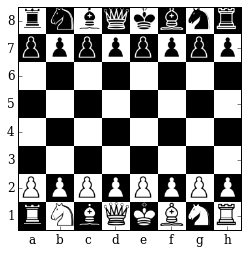
\includegraphics[width=\textwidth]{../img/best_moves/output_17_0.png}
  \begin{itemize}
  \tiny 
  \item 6 layer representation-- Each piece type has one layer.
  \item Friendly pieces are represented as 1. 
  \item Opponent pieces are represented as -1.
  \end{itemize}
  \tiny{
  Similarly we have a 12-layer representation, where each piece type has 2 
layers each. The positions with pieces contain 1s. The alternate layers are 
used for the pieces of each of the players.}

  \end{column}
  \begin{column}{6.3cm}
  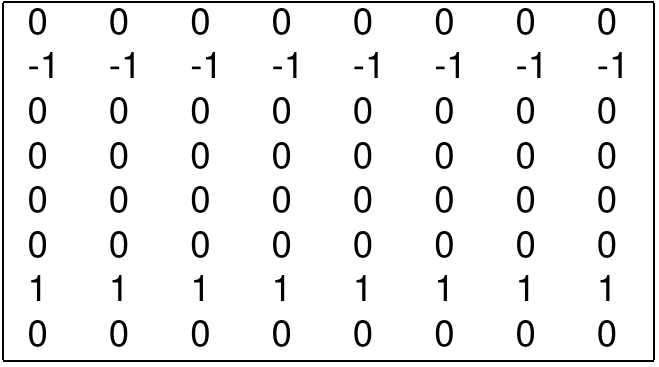
\includegraphics[width=0.5\textwidth, height=2.0cm]{../img/channel1.png}
  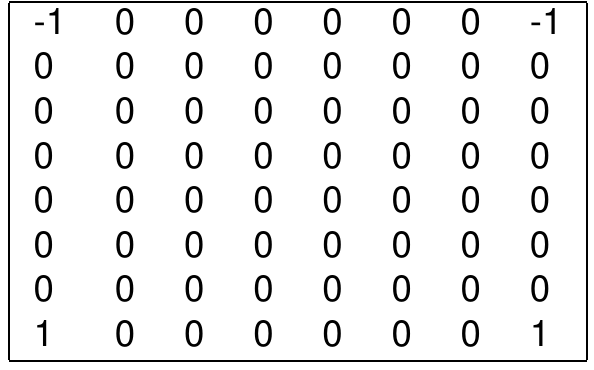
\includegraphics[width=0.5\textwidth]{../img/channel2.png}\\
    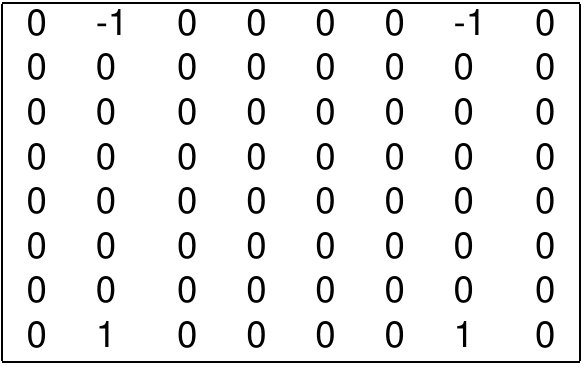
\includegraphics[width=0.5\textwidth]{../img/channel3.png}
  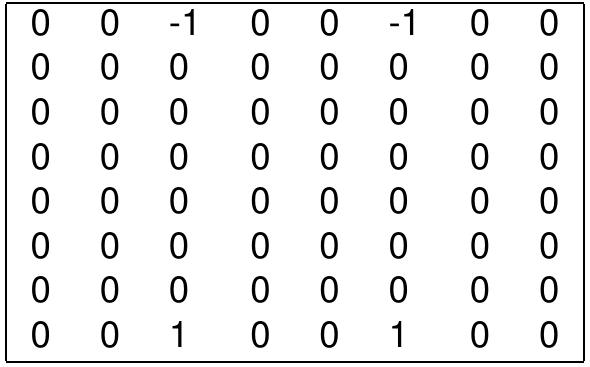
\includegraphics[width=0.5\textwidth]{../img/channel4.png}\\
    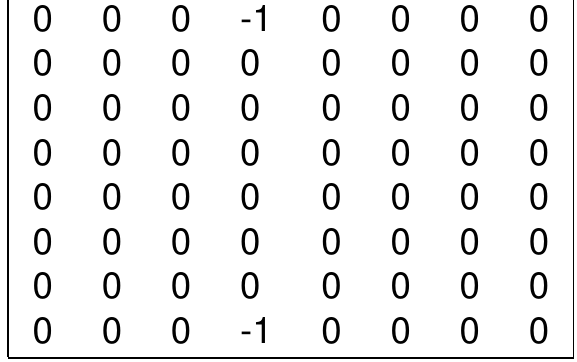
\includegraphics[width=0.5\textwidth]{../img/channel5.png}
  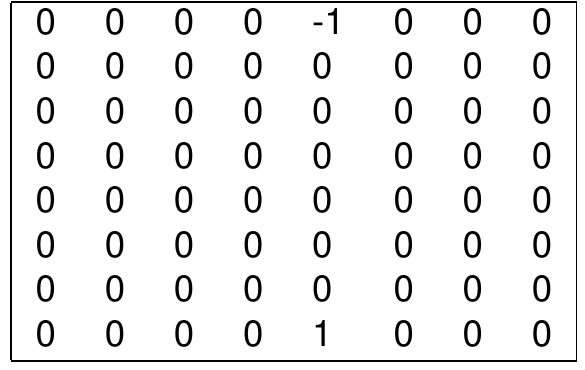
\includegraphics[width=0.5\textwidth]{../img/channel6.png}
  \end{column}

 \end{columns}

\centering

\end{frame}

\begin{frame}{Dataset}{Augmented Bias channels}
\begin{itemize}
 \item There is more information we can provide to our model. We choose to add 
additional bias channels to the 6 or 12 layer data representation.
  \item \textbf{Piece Layer}: While making predictions for the 
\textsc{Move|Piece} network, we add a channel with a 1 in the position of the 
predicted piece. This makes the representation consistent with $P(move | board) 
= P(from|board)\times P(to|from, board)$.
  \item \textbf{Outcome Layer}: We can provide additional information about the 
outcome of the game, so that each move is learned keeping in consideration the 
outcome of the game. The layer adds an addition $1\times 8 \times 8$ channel to 
the data. It contains all 1s for the players who won, all 0s for the players 
who lost, 0.5 for the players who drew. While predicting, we use all 1s in the 
outcome layer.
  \item \textbf{ELO layer}: For each move, we add an additional layer with 
values equal to $\frac{X-MINELO}{MAXELO-MINELO}$, where X is the ELO rating of 
the player who played the move in the datset, MAXELO and MINELO are the 
maximum and minimum ELO ratings of the players in the dataset.
\end{itemize}
 
\end{frame}


%\section{Results and Analysis}
\section{Move Predictor}
\subsection{Description}
\begin{frame}{Piece and Move|Piece Networks}
 \begin{itemize}
  \item We make use of multiple CNNs to predict the 
correct move when presented with a board-- \textsc{Piece} predictor and 
\textsc{Move|Piece} predictors.
  \item $P(move | board) = P(from|board)\times P(to|from, board)$
  \item \textsc{Piece} network predicts the piece. \textsc{Pawn}, 
\textsc{Rook}, \textsc{Knight}, \textsc{Bishop}, \textsc{Queen} and 
\textsc{King} predict the Move|Piece where the piece has been predicted by the 
\textsc{Piece} predictor.
  \item[] 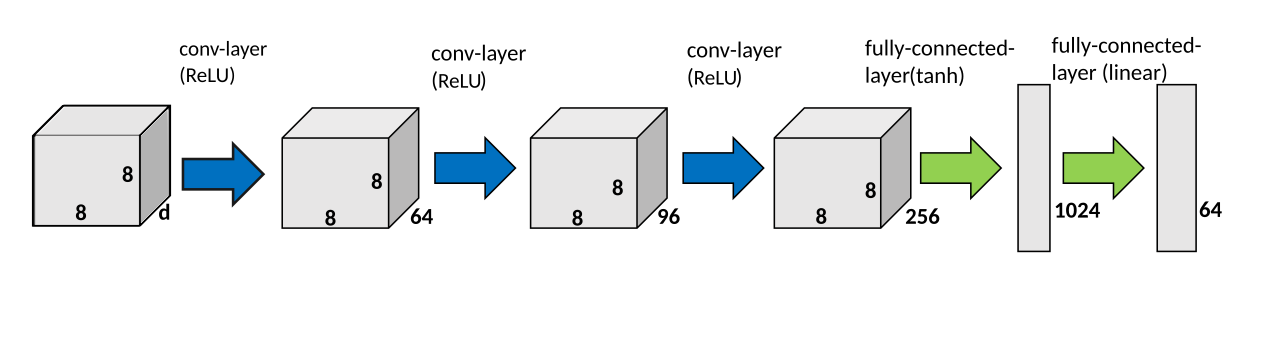
\includegraphics[width=0.8\textwidth,center]{../img/net1.png}
  \item Architecture:
  \begin{itemize}
   \item Convolutional Layer 1: 64 filters of size $3\times 3$ followed by ReLU
    \item Convolutional Layer 2: 96 filters of size $3\times 3$ followed by ReLU
    \item Convolutional Layer 3: 256 filters of size $3\times 3$ followed by 
ReLU
    \item Fully Connected Layer 1: 1024 dimensions
    \item Softmax layer: Outputs a 64-dimensional probability distribution
  \end{itemize}

 \end{itemize}

\end{frame}

\subsection{Training}
\begin{frame}{Training}{Loss function and updates}
\begin{itemize}
 \item Softmax layer outputs the probability of each of the 64 
possibilities as: $p_k=\frac{e^{o_k}}{\sum_i e^{o_i}}$, $o_k$ is the activation 
of the last fully connected layer in the network
  \item Loss is computed using: $L = - \sum_j y_j log p_j$
  \item Gradients for the last layer:
  \begin{align*}
 \frac{\partial L}{\partial o_i} &= -\sum_k y_k\frac{\partial log p_k}{\partial 
o_i} \\
&= -\sum_k y_k \frac{1}{p_k}\frac{\partial p_k}{\partial o_i}\\
&= -y_i(1-p_i) - \sum_{k\neq i} y_k \frac{1}{p_k}(-p_kp_i)\\
&= p_i\bigg(\sum_k y_k\bigg) - y_i\\
&= p_i-y_i
\end{align*}
 where $y_i$ is the actual outcome for $i^{th}$ label while $p_i$ is the 
predicted probability.
\end{itemize}
\end{frame}

\begin{frame}{Training Curves}
\begin{figure}
  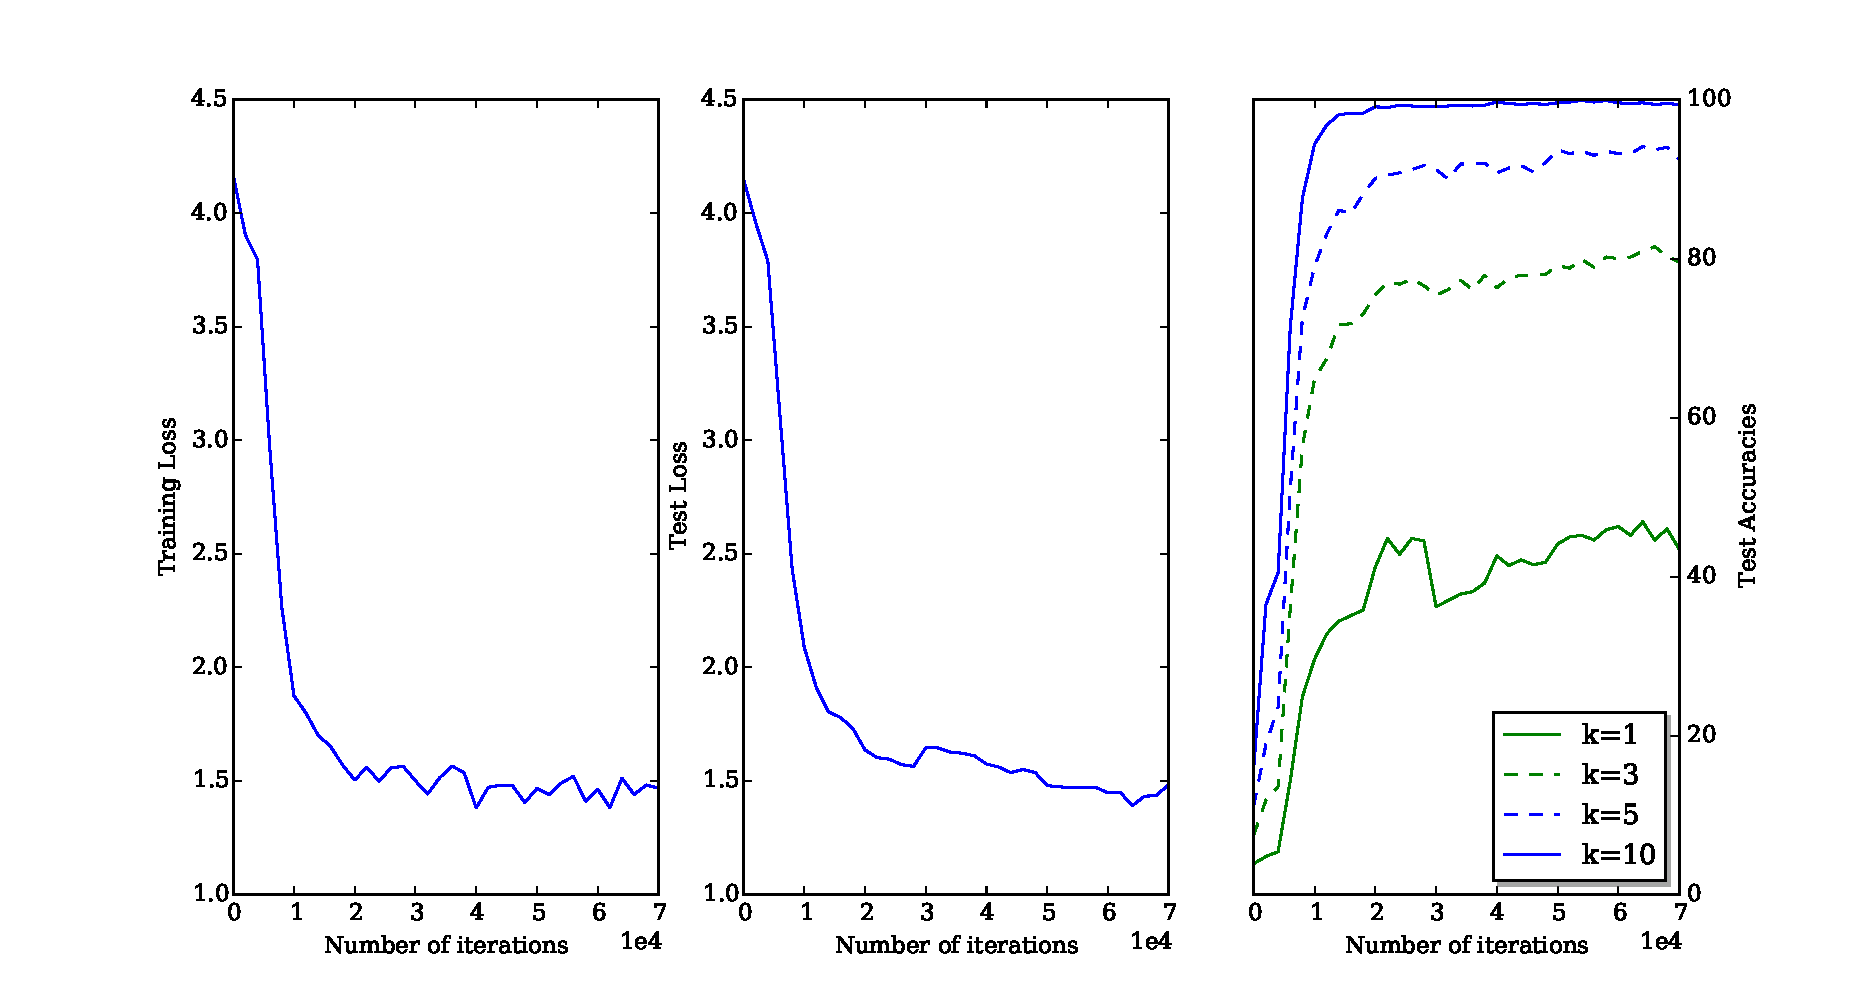
\includegraphics[width=\textwidth,center]{../plots/learning_curve_new.pdf}
  \caption[Variation of the accuracies on test set while training]{
  (a) Softmax-loss on training dataset (b) Softmax-loss on 
testing dataset; (c) Accuracies at k=1,3,5,10 on testing dataset.}
  \label{figure:losses-accuracies}
\end{figure}
\end{frame}

\subsection{Performance}
\begin{frame}
 \frametitle{Accuracies of the \textit{piece} and \textit{move|piece} 
predictors}
\begin{table}[H]
\centering
\begin{tabular}{@{}lllll@{}}
\toprule
\multirow{2}{*}{Model Name} & \multicolumn{4}{c}{Accuracy at k}                 
 
                                                    \\ \cmidrule(l){2-5} 
                            & \multicolumn{1}{c}{k=1} & \multicolumn{1}{c}{k=3} 
& \multicolumn{1}{c}{k=5} & \multicolumn{1}{c}{k=10} \\ \midrule
Piece                       & 56.0                    & 87.9                    
& 95.8                    & 99.5                     \\
Pawn                        & 94.8                    & 100.0                   
& 100.0                   & 100.0                    \\
Rook                        & 58.0                    & 85.2                    
& 93.5                    & 99.6                     \\
Knight                      & 77.3                    & 96.6                    
& 99.3                    & 100.0                    \\
Queen                       & 54.2                    & 81.3                    
& 90.4                    & 98.2                     \\
King                        & 71.7                    & 95.6                    
& 99.6                    & 100.0                    \\ \bottomrule
\end{tabular}
\caption{Test set performance without masking}
\label{table:performance}
\end{table}
\begin{itemize}
 \item Correct prediction in the top-10 predictions almost everytime
 \item The dataset already has multiple labels for even a single board.
 \item We need to analyze more-- Full move predictions, gameplay....
\end{itemize}

\end{frame}

\begin{frame}
 \frametitle{Masking}
 %insert an image to show masking: 2 tables
  %\begin{}
\begin{columns}
 \begin{column}{5cm}
 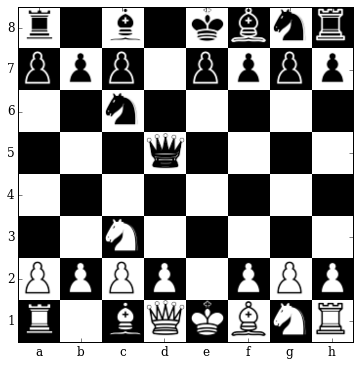
\includegraphics[width=0.8\textwidth]{../img/table_evaluations/output_11_0.png}
  \end{column}
  \begin{column}{5cm}
  \begin{itemize}
   \item Masking is done by zeroing out the probabilities of the illegal 
predictions.
  \item For the \textsc{Piece} predictor, the opponent piece positions and the 
empty positions are zeroed out.
  \item For the \textsc{Move|Piece} predictor, the illegal final positions are 
zeroed out for the respective piece.
  \end{itemize}
 \end{column}

\end{columns}


    \only<2>{
    \begin{table}[]
\centering
\tiny
\label{my-label}
\begin{tabular}{|l|l|l|l|l|l|l|l|}
\hline
0.0000000 & 0.0000001 & 0.0000000 & 0.0000042 & 0.0000001 & 0.0000000 & 
0.0000000 & 0.0000000 \\ \hline
0.0000000 & 0.0000004 & 0.0000000 & 0.0000037 & 0.0000000 & 0.0000016 & 
0.0000010 & 0.0000002 \\ \hline
0.0000001 & 0.0000000 & 0.0000000 & 0.0000001 & 0.0000001 & 0.0000003 & 
0.0000006 & 0.0000005 \\ \hline
0.0000002 & 0.0000000 & 0.0000000 & 0.0000000 & 0.0000000 & 0.0000001 & 
0.0000000 & 0.0000001 \\ \hline
0.0000000 & 0.0000000 & 0.0000000 & 0.0000000 & 0.0000000 & 0.0000000 & 
0.0000000 & 0.0000000 \\ \hline
0.0000000 & 0.0000000 & 0.6692031 & 0.0000003 & 0.0000000 & 0.0000000 & 
0.0000000 & 0.0000000 \\ \hline
0.0017913 & 0.0001493 & 0.0000070 & 0.1242154 & 0.0000000 & 0.0097696 & 
0.0081490 & 0.0008657 \\ \hline
0.0001785 & 0.0000001 & 0.0000146 & 0.0031704 & 0.0000972 & 0.0206326 & 
0.1617075 & 0.0000350 \\ \hline
\end{tabular}
\caption{Unmasked Probability distribution}
\end{table}
    }
    \only<3>{
    \begin{table}[]
\centering
\tiny
\begin{tabular}{|l|l|l|l|l|l|l|l|}
\hline
0.0000000 & 0.0000000 & 0.0000000 & 0.0000000 & 0.0000001 & 0.0000000 & 
0.0000000 & 0.0000000 \\ \hline
0.0000000 & 0.0000000 & 0.0000000 & 0.0000000 & 0.0000000 & 0.0000000 & 
0.0000000 & 0.0000000 \\ \hline
0.0000000 & 0.0000000 & 0.0000000 & 0.0000000 & 0.0000000 & 0.0000000 & 
0.0000000 & 0.0000000 \\ \hline
0.0000000 & 0.0000000 & 0.0000000 & 0.0000000 & 0.0000000 & 0.0000000 & 
0.0000000 & 0.0000000 \\ \hline
0.0000000 & 0.0000000 & 0.0000000 & 0.0000000 & 0.0000000 & 0.0000000 & 
0.0000000 & 0.0000000 \\ \hline
0.0000000 & 0.0000000 & 0.6692101 & 0.0000000 & 0.0000000 & 0.0000000 & 
0.0000000 & 0.0000000 \\ \hline
0.0017914 & 0.0001493 & 0.0000070 & 0.1242167 & 0.0000000 & 0.0097697 & 
0.0081490 & 0.0008658 \\ \hline
0.0001785 & 0.0000000 & 0.0000146 & 0.0031704 & 0.0000972 & 0.0206328 & 
0.1617092 & 0.0000350 \\ \hline
\end{tabular}
\caption{Masked Probability distribution}
\end{table}
    }
\end{frame}

\begin{frame}{Rule Learning}{Performance after masking}
 {\tiny
Let $p$ and $q$ be the distributions before and after masking. We compute two 
distances between both.
\[D_{sq\ euc}(p,q) = ||p-q||^2\]
\[D_{chebyshev}(p,q) = \max_{i}|p_i-q_i|\]
}
\begin{table}
\tiny
\begin{tabular}{@{}llllll@{}}
\toprule
{\bf } & $||p-q||^2$ & $\max_i |p_i-q_i|$& Illegal move& 
\multicolumn{2}{l}{Avg Rank of actual move} \\ \cmidrule(l){5-6} 
{\bf Model}           &        &             &\%age                        & 
unmasked          & masked          \\ \midrule
{\sc Piece}  &     $3.09\times 10^{-8}$ & $4.28\times 10^{-5}$                 
    & 0.0 &2.06342060113 &2.06341424668                   
\\
{\sc Pawn}   &     $1.72\times 10^{-4}$               & $5.82\times 10^{-4}$    
                  & 0.0045 &       1.08001395504 &1.07996844947             
\\
{\sc Rook}   &             $3.74\times 10^{-3}$& $1.37\times 10^{-2}$           
 &   0.72       &2.31513493742 &2.28972185557           
\\
{\sc Knight} &       $1.74\times 10^{-5}$             &     $4.8\times 
10^{-4}$                  &       0.0 & 1.44417866616 &1.44410761652            
  
\\
{\sc Bishop}  &    $3.94\times 10^{-3}$                &  $1.15\times 10^{-2}$  
 
& 0.47                 &  1.83962121376 & 1.82638963959         
\\
{\sc Queen}  &     $5.49\times 10^{-3}$               & $1.89\times 10^{-2}$ &  
   1.23                &                   2.52614094756 &2.47512457486  
\\
{\sc King}   &    $3.35\times 10^{-3}$                &   $3.82\times 10^{-3}$ 
&       0.33            &      1.59097552371 & 1.5873805164        
\\ \bottomrule
\end{tabular}
\end{table}

 \begin{itemize}
  \item Observe that there is not much difference between the probability 
distributions before and after masking.	
  \item Piece selector model doesn't predict any illegal piece positions.
  \item There are no incorrect moves predicted for knights.
 \end{itemize}

\end{frame}


\begin{frame}
 \frametitle{Performance after Masking}
 In the table, the accuracies of each of the models is compared before 
and after masking for the set of $314,740$ board positions.
 \begin{table}
\centering
\begin{tabular}{@{}lll@{}}
\toprule
\multirow{2}{*}{Model} & \multicolumn{2}{l}{Percentage Accuracy} \\ 
\cmidrule(l){2-3} 
                       & before masking      & after masking     \\ \midrule
Piece                  & 56.11               & 56.11             \\
Pawn                   & 53.60               & 53.60             \\
Rook                   & 50.98               & 51.26             \\
Knight                 & 72.77               & 72.77             \\
Bishop                 & 59.89               & 60.13             \\
Queen                  & 47.99               & 48.42             \\
King                   & 64.49               & 64.76             \\ 
\bottomrule
\end{tabular}
\caption{Accuracies before and after masking.}
\end{table}
\end{frame}

\begin{frame}
 \frametitle{Evaluating performance of full move prediction}
 
\only<1>{
 \begin{figure}
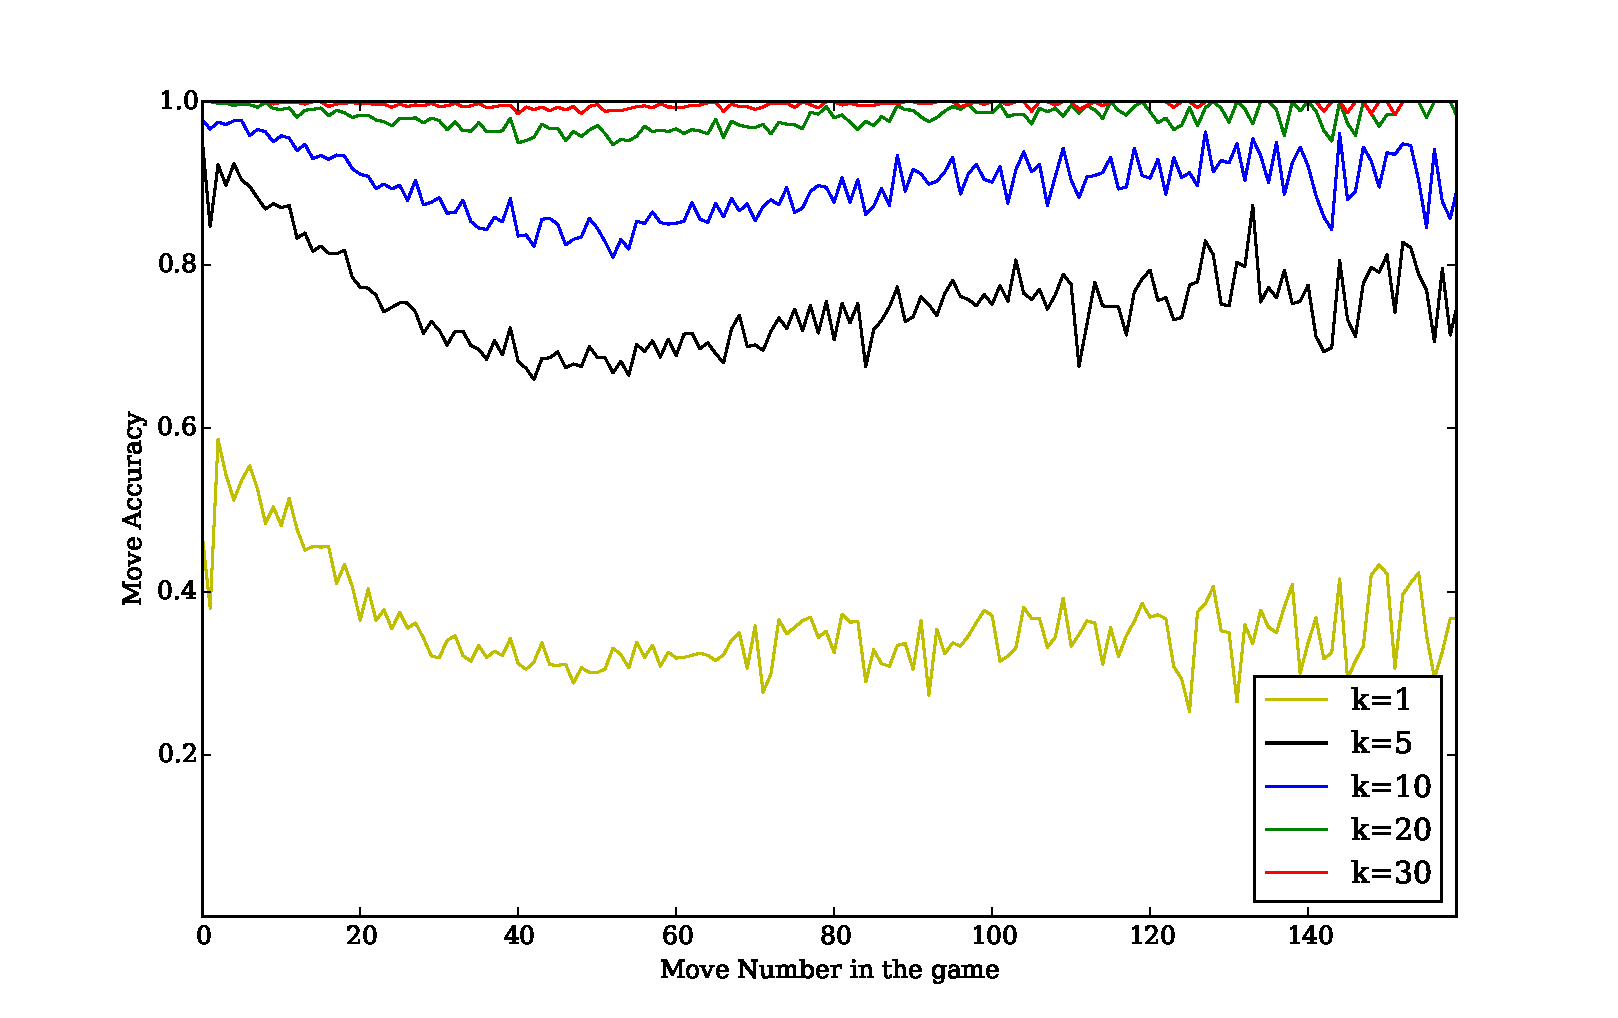
\includegraphics[width=0.8\textwidth,center]{../plots/accuracy_new.pdf}
\caption[Variation of accuracies with move number]{Average accuracies at 
different move numbers in test dataset games for top k 
predictions (k=1,5,10,30).}
\label{figure:gameplay1}
\end{figure}
}
\only<2>{
\begin{figure}
  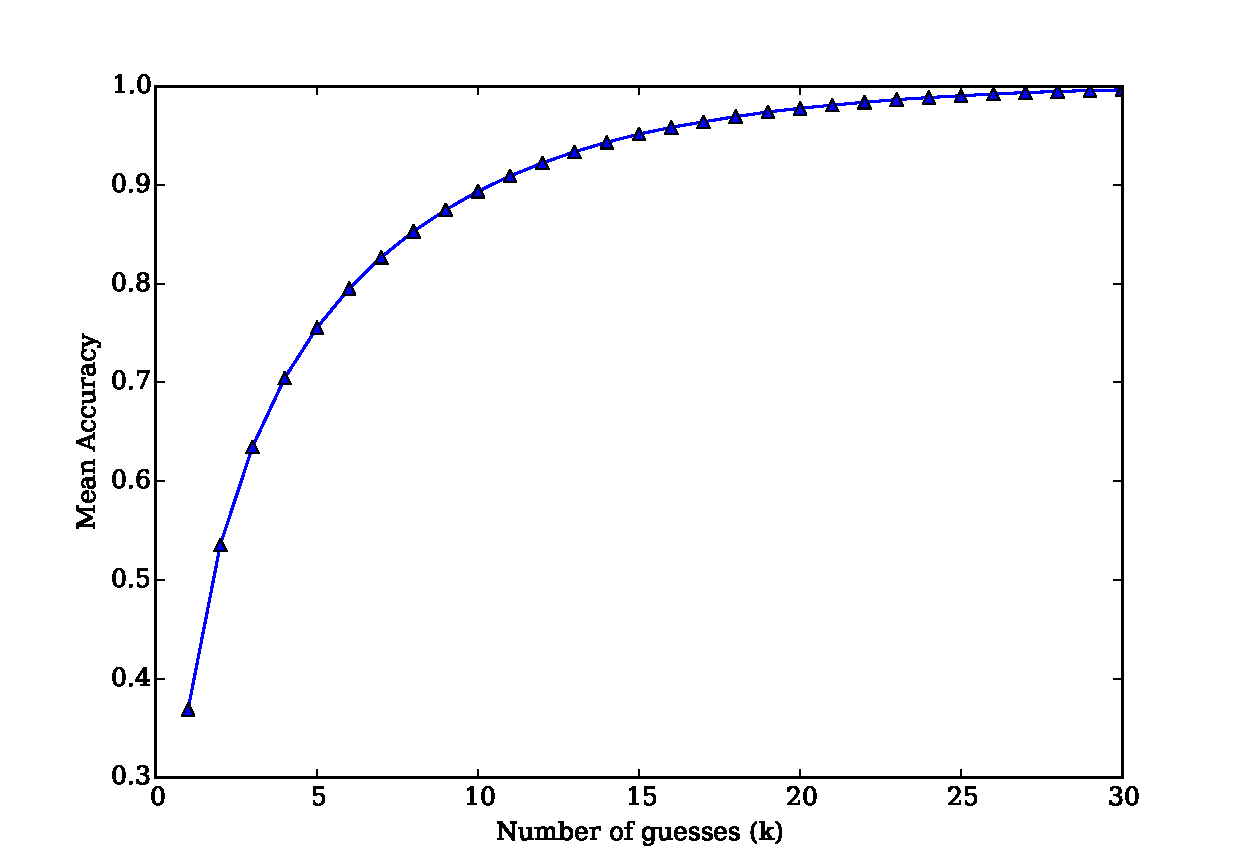
\includegraphics[width=0.8\textwidth,center]{../plots/accuracy2_new.pdf}
  \caption[Variation of Top-k accuracy with k]{
  Plot of the variation of mean accuracy of the actual move lying in the 
top-k predictions with k (the number of guesses).}
  \label{figure:gameplay2}
\end{figure}
}
\end{frame}

\subsection{Case studies}
\begin{frame}{Case studies}{Predictions for Opening Move}
 \begin{columns}[c]
 \begin{column}{4cm}
 \begin{figure}[H]
 \centering
    \begin{subfigure}[t]{\textwidth}
	
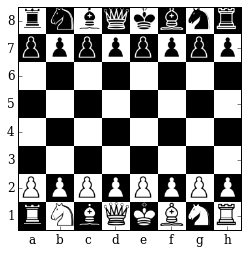
\includegraphics[width=0.75\textwidth]{../img/best_moves/output_17_0.png}
        \label{figure:initialboarda}
    \end{subfigure}%
  \\
    \begin{subfigure}[t]{\textwidth}
        
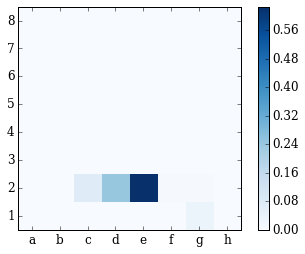
\includegraphics[width=0.9\textwidth]{../img/best_moves/output_12_0.png}
        \caption{$P_{\textsc{piece}}(B)$}
        \label{figure:initialboardb}
%         Predicted probability distribution\\
%         for the ``from'' position\\
%         predicted by \textsc{PIECE} network}
    \end{subfigure}
\caption[Predictions for initial board position]{Predictions for initial board 
position}
\end{figure}
\end{column}
\begin{column}{6cm}
 \begin{table}[]
 \tiny
\centering
\begin{tabular}{@{}llll@{}}
\toprule
Move & $P_{\textsc{piece}}$ & No. of times played & \%age times 
played \\ 
\midrule
All  & 1.0000000             & 4970725                & 100.00\%           \\ 
\midrule
e2e4 & 0.6088475             & 2221439                & 44.7\%             \\
d2d4 & 0.2467637             & 1618291                & 32.6\%             \\
c2c4 & 0.0725896             & 286295                 & 5.8\%              \\
g1f3 & 0.0334573             & 334741                 & 6.7\%              \\
e2e3 & 0.0171652             & 62744                  & 1.3\%              \\
f2f4 & 0.0059381             & 67248                  & 1.4\%              \\
g2g3 & 0.0052637             & 93072                  & 1.9\%              \\
b1c3 & 0.0021147             & 98306                  & 2\%                \\
b2b3 & 0.0013837             & 64692                  & 1.3\%              \\
c2c3 & 0.0013727             & 17449                  & 0.4\%              \\
d2d3 & 0.0011852             & 43647                  & 0.9\%              \\
g2g4 & 0.0008549             & 11245                  & 0.2\%              \\
h2h3 & 0.0007792             & 5814                   & 0.1\%              \\
b2b4 & 0.0007009             & 13761                  & 0.3\%              \\
a2a3 & 0.0005240             & 5843                   & 0.1\%              \\
g1h3 & 0.0002781             & 3875                   & 0.1\%              \\
b1a3 & 0.0002716             & 1013                   & 0\%                \\
h2h4 & 0.0002087             & 7216                   & 0.1\%              \\
a2a4 & 0.0002071             & 4967                   & 0.1\%              \\
f2f3 & 0.0000310             & 9067                   & 0.2\%              \\ 
\bottomrule
\end{tabular}
\caption{The percentage of times a certain opening 
was played according the the opening database on 
\url{http://www.ficsgames.org/openings.html}. }
\label{table:initialboard}
\end{table}
\end{column}
\end{columns}

\end{frame}
\begin{frame}{Case studies}{Checkmate in 1 and Detecting a check}
\begin{figure}[H] 
  \centering
    \begin{subfigure}[t]{0.3\textwidth}
        \centering
        
      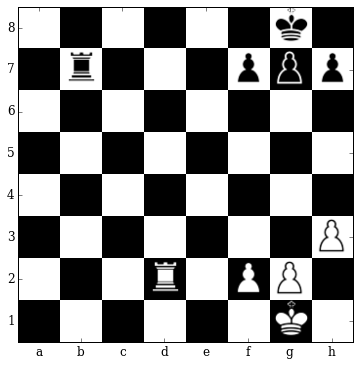
\includegraphics[width=\textwidth]{../img/best_moves/output_21_0.png}
        \caption{There is a check and mate 
possible in one move of the white.}
    \end{subfigure}
    ~
    \begin{subfigure}[t]{0.3\textwidth}
        \centering
        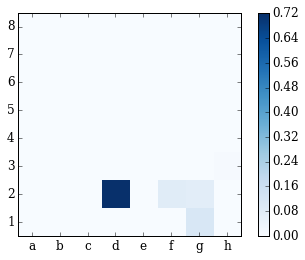
\includegraphics[width=\textwidth]{../img/best_moves/output_21_2.png}
        \caption{$P_{\textsc{piece}}(B)$}
    \end{subfigure}
    ~
    \begin{subfigure}[t]{0.3\textwidth}
        \centering
        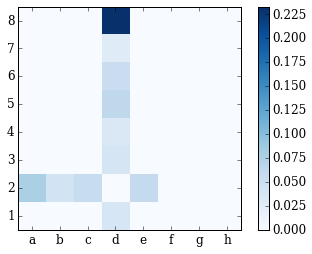
\includegraphics[width=\textwidth]{../img/best_moves/output_21_6.png}
        \caption{$P_{\textsc{rook}}(B, d2)$}
    \end{subfigure}
\label{figure:checkmating}
\end{figure}

\begin{figure}[H]
  \centering
    \begin{subfigure}[t]{0.3\textwidth}
        \centering
        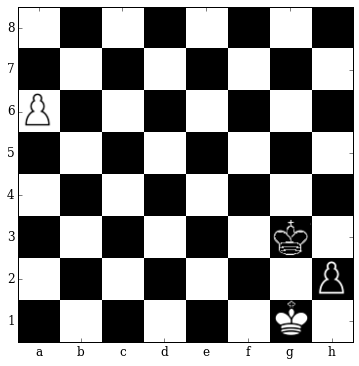
\includegraphics[width=\textwidth]{../img/best_moves/output_24_0.png}
        \caption{The white king is under check}
    \end{subfigure}
    ~
    \begin{subfigure}[t]{0.3\textwidth}
        \centering
        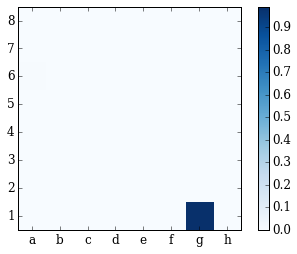
\includegraphics[width=\textwidth]{../img/best_moves/output_24_2.png}
        \caption{$P_{\textsc{piece}}(B)$}
    \end{subfigure}
    ~
  \centering
    \begin{subfigure}[t]{0.3\textwidth}
        \centering
        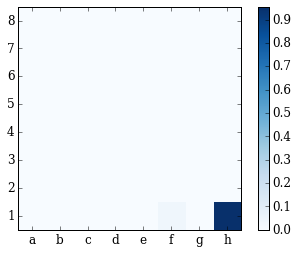
\includegraphics[width=\textwidth]{../img/best_moves/output_24_6.png}
        \caption{$P_{\textsc{king}}(B, g1)$}
    \end{subfigure}
\label{figure:check-detection}
\end{figure}

 
\end{frame}
\begin{frame}{Case Studies}{En Passant and Castling}
\begin{figure}[H] 
  \centering
    \begin{subfigure}[t]{0.3\textwidth}
        \centering
        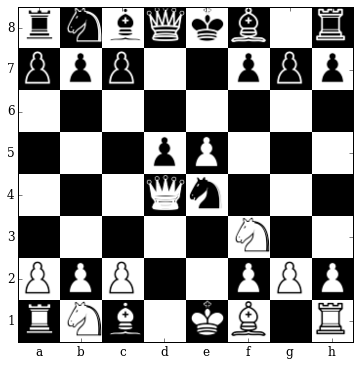
\includegraphics[width=\textwidth]{../img/best_moves/output_38_0.png}
        \caption{The d-pawn just moved 2 steps}
    \end{subfigure}
    ~
    \begin{subfigure}[t]{0.3\textwidth}
        \centering
        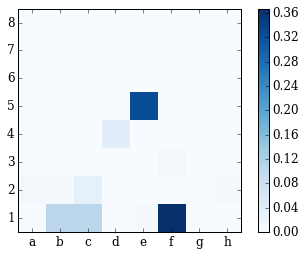
\includegraphics[width=\textwidth]{../img/best_moves/output_38_2.png}
        \caption{$P_{\textsc{piece}}(B)$}
    \end{subfigure}
    ~
  \centering
    \begin{subfigure}[t]{0.3\textwidth}
        \centering
        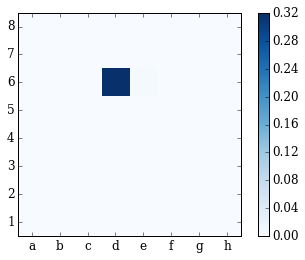
\includegraphics[width=\textwidth]{../img/best_moves/output_38_6.png}
        \caption{$P_{\textsc{pawn}}(B, e5)$}
    \end{subfigure}%
\end{figure}

\begin{figure}[H]
  \centering
    \begin{subfigure}[t]{0.3\textwidth}
        \centering
        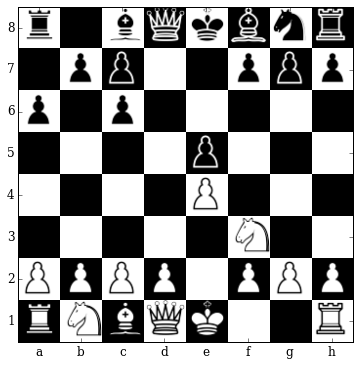
\includegraphics[width=\textwidth]{../img/best_moves/output_22_0.png}
        \caption{Board position. Castling is one of the favorable moves 
available.}
    \end{subfigure}
    ~
    \begin{subfigure}[t]{0.3\textwidth}
        \centering
        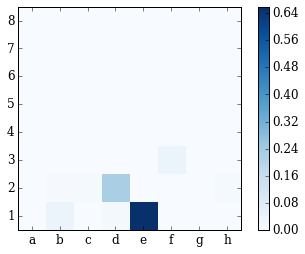
\includegraphics[width=\textwidth]{../img/best_moves/output_22_2.png}
        \caption{$P_{\textsc{piece}}(B)$}
    \end{subfigure}
    ~
  \centering
    \begin{subfigure}[t]{0.3\textwidth}
        \centering
        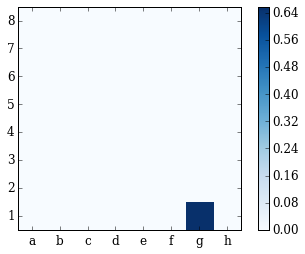
\includegraphics[width=\textwidth]{../img/best_moves/output_22_6.png}
        \caption{$P_{\textsc{king}}(B, e1)$}
    \end{subfigure}%
\end{figure}
\end{frame}

\begin{frame}{Case Study}{Carlsen vs Anand, Game 6, 2014 World 
Championship}
 \begin{columns}[c]
 \begin{column}{4cm}
  \begin{figure}[H]
  \centering
  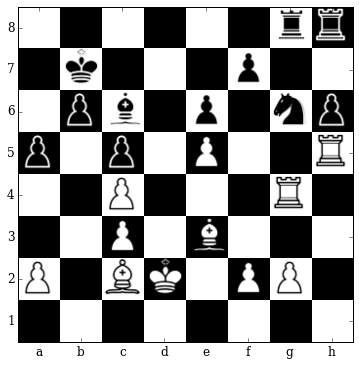
\includegraphics[width=\textwidth]{../img/best_moves/vishy-magnus.png}
  \caption[Middle game case study]{Black to move. 26th move.}
\end{figure}
    
  \end{column}
\begin{column}{6cm}
\uncover<2->{
\begin{table}[H]
\tiny
\centering
\begin{tabular}{@{}lll@{}}
\cmidrule(r){1-2}
Move & Predicted Probability &                                  \\ 
\cmidrule(r){1-2}
g8d8 & 0.252880722284        &                                  \\
g8g7 & 0.148237019777        &                                  \\
g6e5 & 0.13111974299         & \uncover<3->{Expected Move}           \\
b7c7 & 0.0660261586308       &                                  \\
h8h7 & 0.0471959412098       &                                  \\
c6g2 & 0.0403394699097       &                                  \\
c6e8 & 0.0358173549175       &                                  \\
g8c8 & 0.0323895104229       &                                  \\
b7c8 & 0.0302288047969       &                                  \\
c6d7 & 0.0250529013574       &                                  \\
a5a4 & 0.0231475103647       & \uncover<3->{Anand's actual move} \\
g6e7 & 0.0229441132396       &                                  \\
b7a6 & 0.0208601523191       &                                  \\
g8a8 & 0.0198916308582       &                                  \\
b7b8 & 0.0190593209118       &                                  \\
c6a4 & 0.0153007712215       &                                  \\
g6f8 & 0.0150824002922       &                                  \\
g8f8 & 0.0115283448249       &                                  \\
g8e8 & 0.00727259740233      &                                  \\
b7a7 & 0.00666899653152      &                                  \\ 
\cmidrule(r){1-2}
\end{tabular}
\caption{Possible moves after the mistake by Carlsen in Move 26}
\label{table:vishy-carlsen}
\end{table}
}
\end{column}
\end{columns}

\uncover<4->{\small
 A tweet said-- \textit{``Wow 26...Ne5! and black is 
winning....Anand plays 26...a4? Whats going on :) \#CarlsenAnand''}}
 \end{frame}


\section{Evaluation Function}
\begin{frame}{Evaluation function}
\begin{tiny}
\begin{itemize}
 \item Given a game in the dataset, consider the following assignment:
 \[V(b_{t_{final}}) = \begin{cases}
1 \text{ , if White has won}\\
0 \text{ , if it is a draw}\\
-1 \text{ , if Black has won}
\end{cases}\]
\item According to the recursive rule the discounted reward 
for a board at time $t$ 
into the game is:
\[V(t) = \gamma V(t+1) , \forall t<t_{final}\]
\item Use the following rule moving up into the game:
\[V(b_{t_{final}-i}) = \begin{cases}
		\gamma^{i} \text{ , if white won eventually}\\
                -\gamma^{i} \text{ , if black won eventually}\\
                0 \text{ , if the game was a draw}\\
               \end{cases}\]
\[V(b'_{t_{final}-i}) = \begin{cases}
		-\gamma^{i} \text{ , if white won eventually}\\
                \gamma^{i} \text{ , if black won eventually}\\
                0 \text{ , if the game was a draw}\\
               \end{cases}\]
where $b_{t_{final}-i}$ is the board (as it appears to the white player) $i$ 
steps away from the finish, while $b'_{t_{final}-i}$ is the rotated board with 
flipped colors $i$ steps away from the finish.
\item In this way, each board in the dataset is assigned an evaluation.
\end{itemize}
\end{tiny}
\end{frame}

\subsection{Examples}
\begin{frame}{Evaluation Function}{Training}
\begin{itemize}
  \item[] 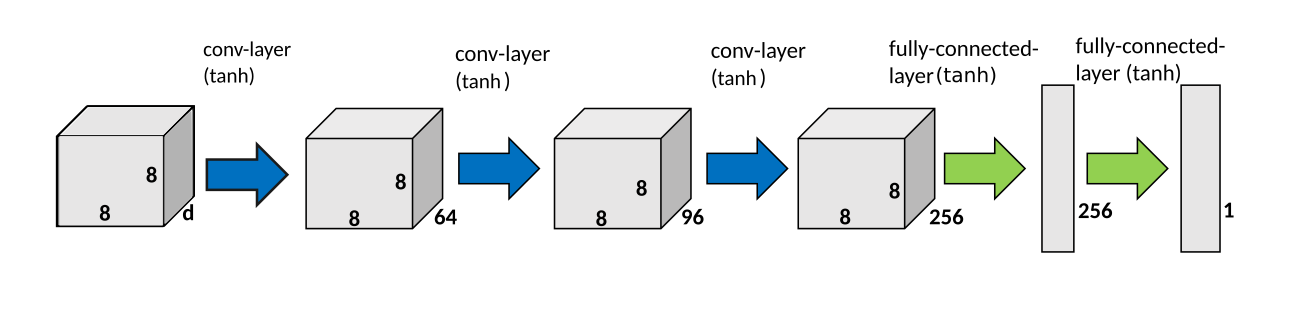
\includegraphics[width=.90\textwidth,center]{../img/net3.png}
  \item Modeled as a regression problem with the evaluation value as the 
dependent variable and the board images as the regressors.
  \item Loss function: \[L = \frac{1}{2}(f(x)-y)^2\] where $x$ is the value at 
the last fully-connected layer in the network and $f$ is the activation 
function (tanh in our 
case).
\item Simply the gradient looks like:
\[\frac{\partial L}{\partial x} = (f(x)-y)\frac{\partial f(x)}{\partial x}\]
\end{itemize}
\end{frame}


\begin{frame}{Evaluation function}{Examples}
\only<1>{
\begin{figure}[H] 
  \centering
    \begin{subfigure}[t]{0.3\textwidth}
        \centering
        
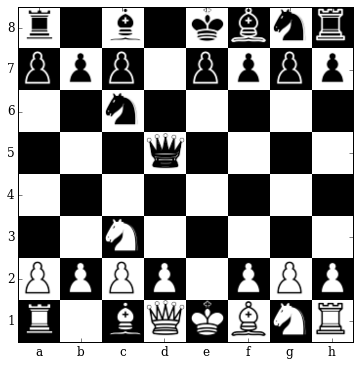
\includegraphics[width=\textwidth]{../img/table_evaluations/output_11_0.png}
        \caption{Board position (White to move)}
    \end{subfigure}%
    ~
    \begin{subfigure}[t]{0.3\textwidth}
        \centering
        
    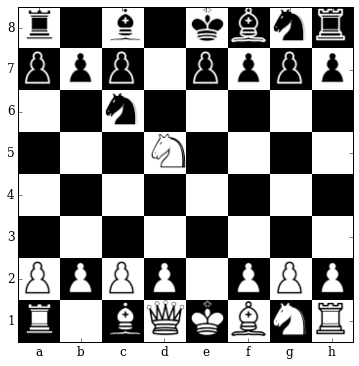
\includegraphics[width=\textwidth]{../img/table_evaluations/output_11_2.png}
        \caption{Move: c3d5\\
        $V_{\gamma=0.7}=0.0545$}
    \end{subfigure}
   ~
    \begin{subfigure}[t]{0.3\textwidth}
        \centering
        
    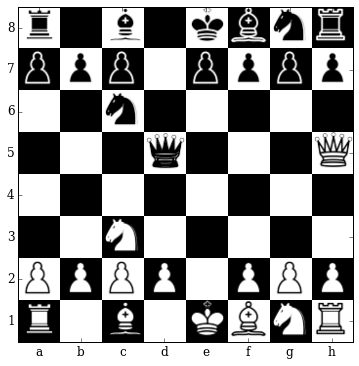
\includegraphics[width=\textwidth]{../img/table_evaluations/output_11_4.png}
        \caption{Move: d1h5\\
        $V_{\gamma=0.7}=0.0144$}
    \end{subfigure}
    \end{figure}
}
\only<2>{
    \begin{figure}[H]
  \centering
    \begin{subfigure}[t]{0.3\textwidth}
        \centering
        
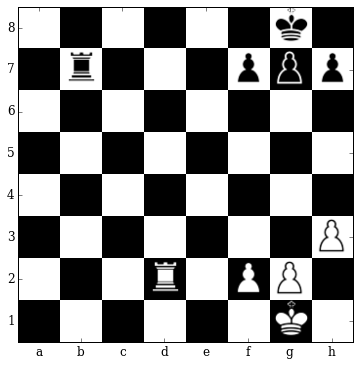
\includegraphics[width=\textwidth]{../img/table_evaluations/output_12_0.png}
        \caption{Board position (White to move)}
    \end{subfigure}
    ~
    \begin{subfigure}[t]{0.3\textwidth}
        \centering
        
    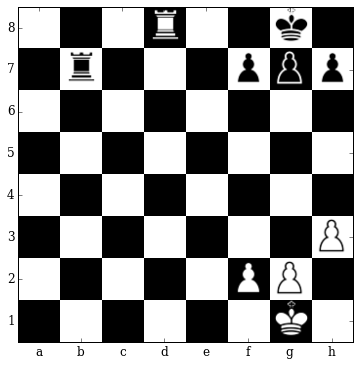
\includegraphics[width=\textwidth]{../img/table_evaluations/output_12_2.png}
        \caption{Move: d2a8\\
        $V_{\gamma=0.7}=0.0543$}
    \end{subfigure}
    ~
    \begin{subfigure}[t]{0.3\textwidth}
        \centering
        
    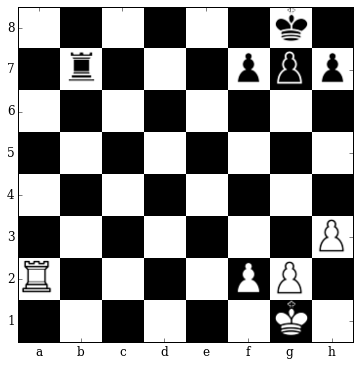
\includegraphics[width=\textwidth]{../img/table_evaluations/output_12_4.png}
        \caption{Move: d2a2\\
        $V_{\gamma=0.7}=0.0177$}
    \end{subfigure}
\end{figure}
}
\only<3>{
\begin{figure}[H] 
  \centering
    \begin{subfigure}[t]{0.3\textwidth}
        \centering
        
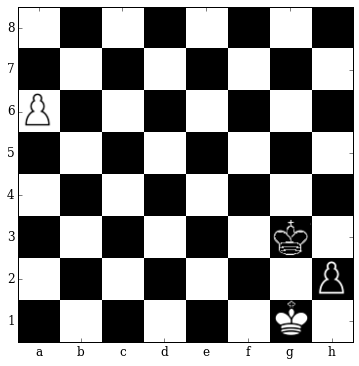
\includegraphics[width=\textwidth]{../img/table_evaluations/output_15_0.png}
        \caption{Board position (White to move)}
    \end{subfigure}
    ~
    \begin{subfigure}[t]{0.3\textwidth}
        \centering
        
    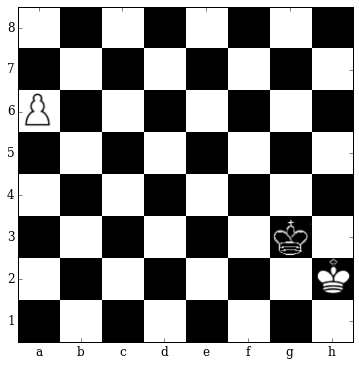
\includegraphics[width=\textwidth]{../img/table_evaluations/output_15_2.png}
        \caption{Move: g1h2 \\
        $V_{\gamma=0.7}=0.0216$}
    \end{subfigure}
    ~
    \begin{subfigure}[t]{0.3\textwidth}
        \centering
        
    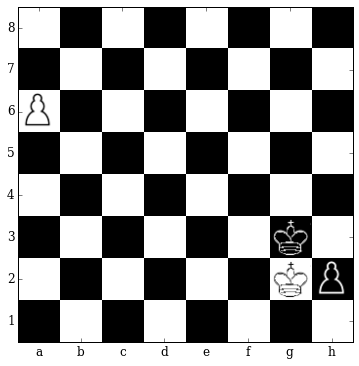
\includegraphics[width=\textwidth]{../img/table_evaluations/output_15_4.png}
        \caption{Move: g1g2 \\
        $V_{\gamma=0.7}=0.0084$}
    \end{subfigure}
\end{figure}
}
\end{frame}

\begin{frame}{Evaluation function}{Correlation with the Material heuristic}
\begin{itemize}
 \item We compare the learned evaluation function with the material heuristic 
values of the boards in our dataset.\\
$V_{\textsc{MATERIAL}}(board) = 1 \times (P-P') + 3 \times (N-N')+ 3 
\times (B-B') + 5 \times (R-R')+ 9 \times (Q-Q')$
where the values of P, N, B, R and Q come from:
\begin{table}[H]
\tiny
\centering
\begin{tabular}{@{}llllll@{}}
\toprule
{\bf Piece} & Pawn & Rook & Knight  & Bishop & Queen \\ \midrule
{\bf Value} & 1    & 5    & 3	    & 3      & 9     \\ \bottomrule
\end{tabular}
\end{table}
\item We compute the correlation of the two evaluation 
functions-- $V_{\gamma=0.7}$ (learned by our model) and $V_{\textsc{MATERIAL}}$.
\uncover<2->{
  \item[] 
  \begin{figure}[H]
 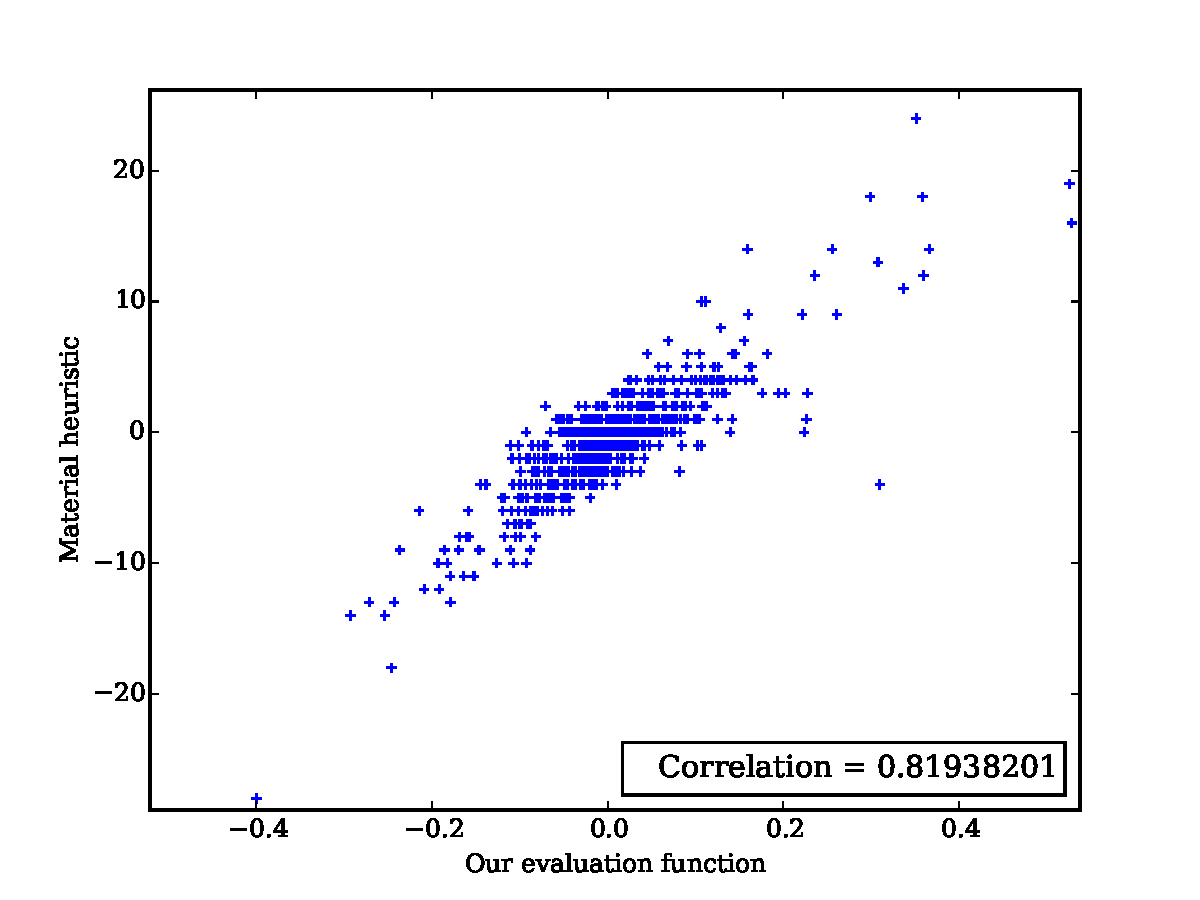
\includegraphics[width=0.6\textwidth]{../plots/correlation_eval.pdf}
\label{figure:correlation}
\end{figure}}
\end{itemize}
 
\end{frame}

\begin{frame}{Evaluation function}{Correlation--Examples}
\begin{figure}[h]
  \centering
    \begin{subfigure}[t]{0.3\textwidth}
        \centering
        
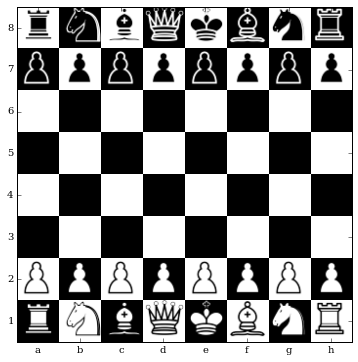
\includegraphics[width=\textwidth]{../img/table_evaluations/output_35_0.png}
        \centering
        \caption{$V_{\gamma=0.7} = 0.0015796$\\  
$V_{\textsc{MATERIAL}}= 0.0 $}
  \label{figure:correlation2d}
    \end{subfigure}
    ~
    \begin{subfigure}[t]{0.3\textwidth}
        \centering
        
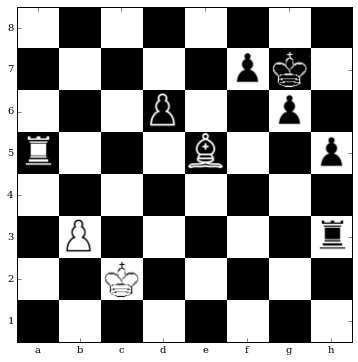
\includegraphics[width=\textwidth]{../img/table_evaluations/output_33_0.png}
         \caption{$V_{\gamma=0.7} = -0.0748723$\\  
$V_{\textsc{MATERIAL}}= -6.0 $}
    \end{subfigure}
    
    \begin{subfigure}[t]{0.3\textwidth}
        \centering
        
    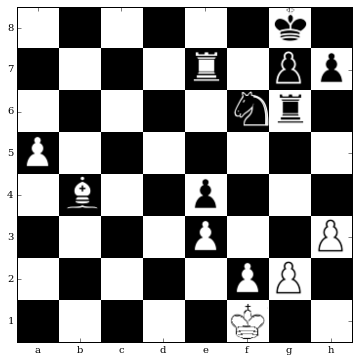
\includegraphics[width=\textwidth]{../img/table_evaluations/output_34_0.png}
         \caption{$V_{\gamma=0.7} = 0.0902274$\\  
$V_{\textsc{MATERIAL}}= 2.0 $}
    \end{subfigure}
    ~
    \begin{subfigure}[t]{0.3\textwidth}
        \centering
        
    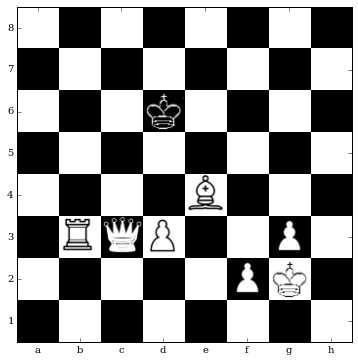
\includegraphics[width=\textwidth]{../img/table_evaluations/output_36_0.png}
         \caption{$V_{\gamma=0.7} = 0.302926$\\  
$V_{\textsc{MATERIAL}}= 20.0 $}
    \label{figure:correlation2d}
    \end{subfigure}
\end{figure} 
\end{frame}

\subsection{Game Trajectories}
\begin{frame}{Game Trajectories}
\begin{figure}[H]
 \only<1>{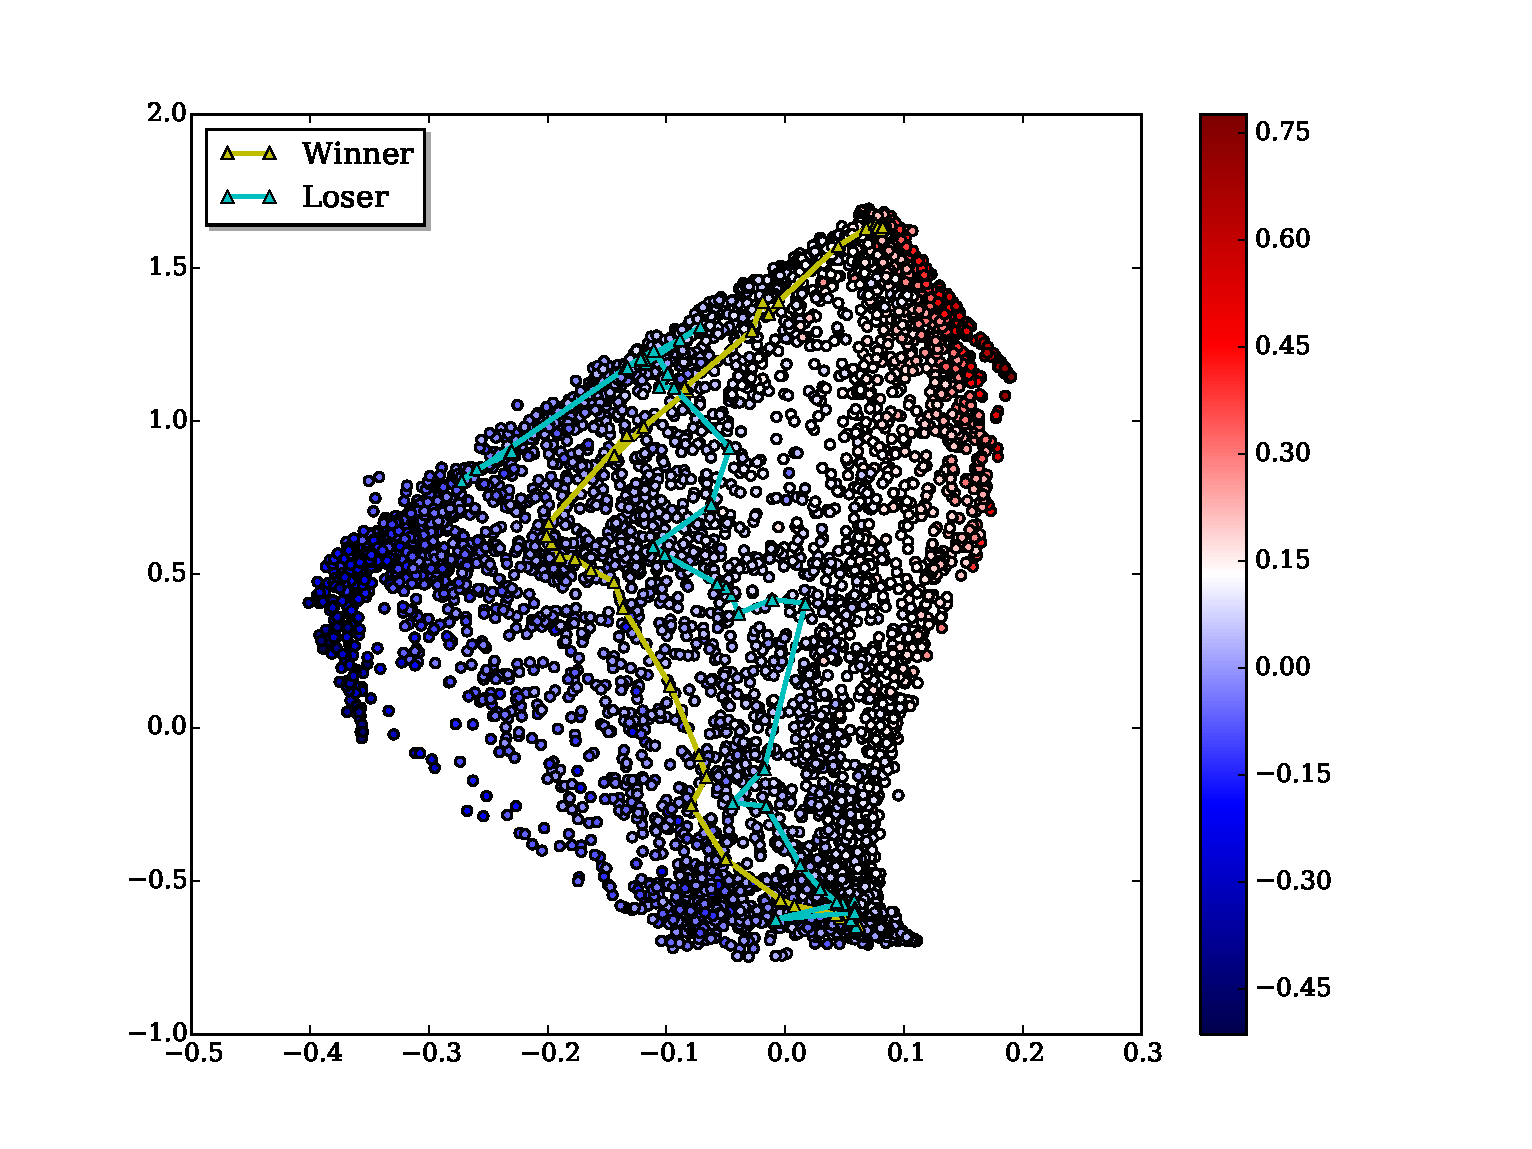
\includegraphics[width=0.85\textwidth]{../plots/board_evals_win.pdf}}
 \only<2>{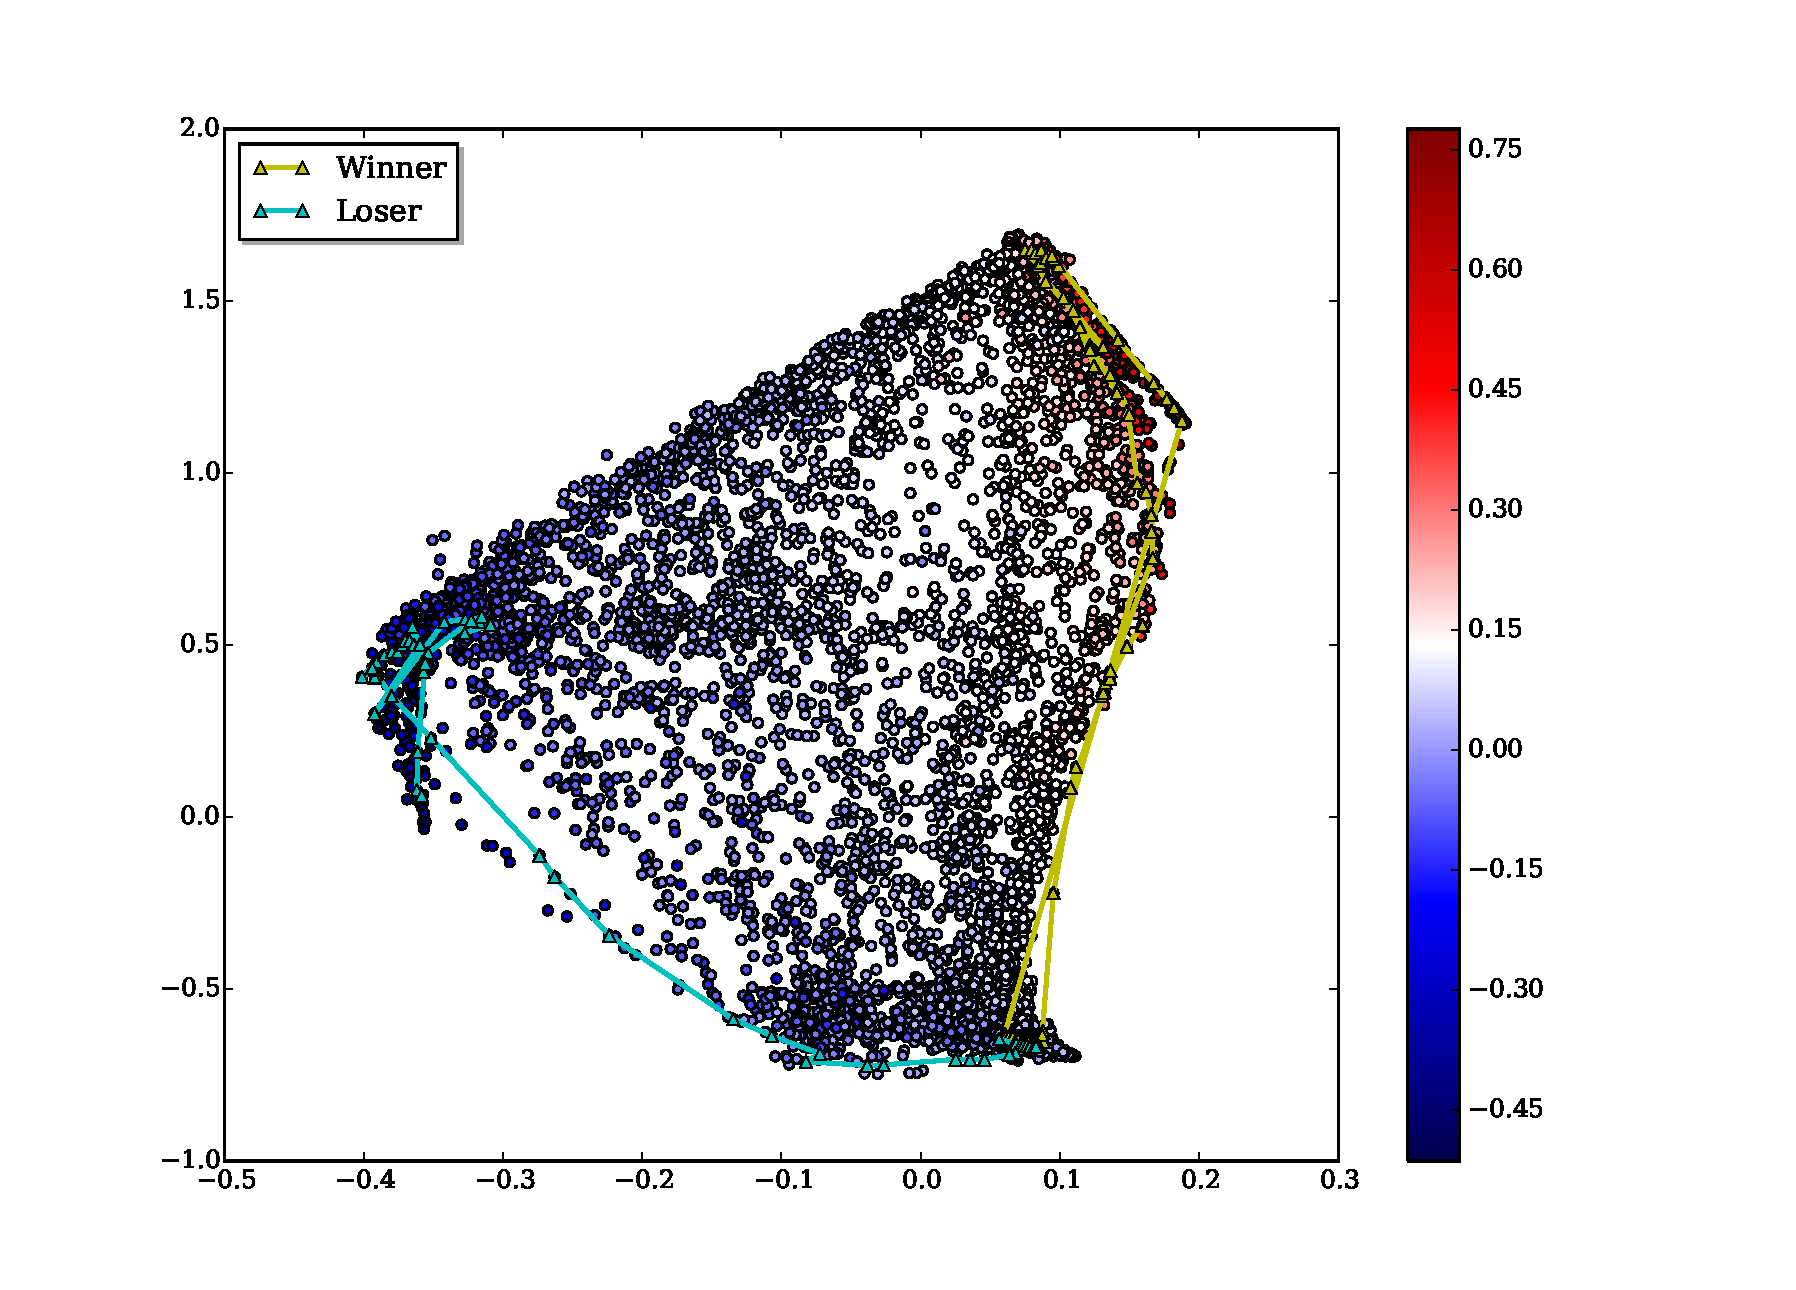
\includegraphics[width=0.89\textwidth]{../plots/board_evals_win2.pdf}}
 \caption[Game Trajectories]{t-SNE embedding of the activations at the last 
fully connected layer of the board evaluation CNN. The red end is the set of 
boards close to winning, the blue end is the set of boards close to losing 
a game. We plot a game on the embedding. The winner(yellow) ends on the red 
side of the embedding while the loser(cyan) ends on the blue side of the 
embedding}
\end{figure}
\end{frame}

\section{Gameplay}
\begin{frame}[fragile]{Gameplay}
\begin{itemize}
 \item Use the predictions and evaluations made by the models discussed to play 
a game of chess
 \item Choosing a move:
 \begin{itemize}
  \item Top Move Method: Choose the piece with the highest 
predicted probability, and then choose the position to move the piece to using 
the $move|piece$ model
\only<2>{
\begin{tiny}
\begin{algorithm}[H]
\tiny
\begin{algorithmic}[1]
 	\State initial\_pos = argmax($P_{piece}(board)$)\;
   	\State piece\_type = getType(initial\_pos)\;
   	\State final\_pos = \funccall{argmax}($P_{move,piece\_type}(board)$)\;
   	\Return chess\_coords(initial\_pos)+chess\_coords(	final\_pos)\;
\end{algorithmic}
\caption{Top-move method}
\label{alg:topmove}
\end{algorithm}
\end{tiny}
 }
  \only<3->{
 \item Top Prob Method: Choose the move with the maximum joint probability-- 
$P(move | board ) = P(piece | board )\times 
P(final\_position|piece, board)$
  }
  \only<4>{
  \begin{algorithm}[H]
  \tiny
 \begin{algorithmic}[1]
 	\State piece\_dist = $P_{piece}(board)$
   	\State cumulative\_dist = \funccall{zeros}(64,64)
   	\For {$0\leq i<64$}
   		\If {$board[i/8,i\% 8]\neq 0$}
   			\State piece\_type=\funccall{getType}(i)
   			\State move\_distr = $P_{move,piece\_type}(board)$ * 
piece\_distr[i]
   			\State cumulative\_distr[i] = move\_distr
   		\EndIf
   	\EndFor
   	\State initial\_pos, final\_pos = \funccall{argmax}(cumulative\_distr)
   	\Return \funccall{chess\_coords}(initial\_pos)+\funccall{chess\_coords}	
(	final\_pos)
 \end{algorithmic}
 \caption{Top-prob method}
 \label{alg:topprob}
\end{algorithm}
  }
 \end{itemize}
\end{itemize}
\end{frame}

\begin{frame}{Gameplay}{Negamax}
\begin{itemize}
 \item A modified version of minimax algorithm
 \item It utilizes the same subroutine for the Min player and the Max 
player at each step, passing on the negated score following the rule:
\[max(a,b) = -min(-a,-b)\]
\end{itemize}

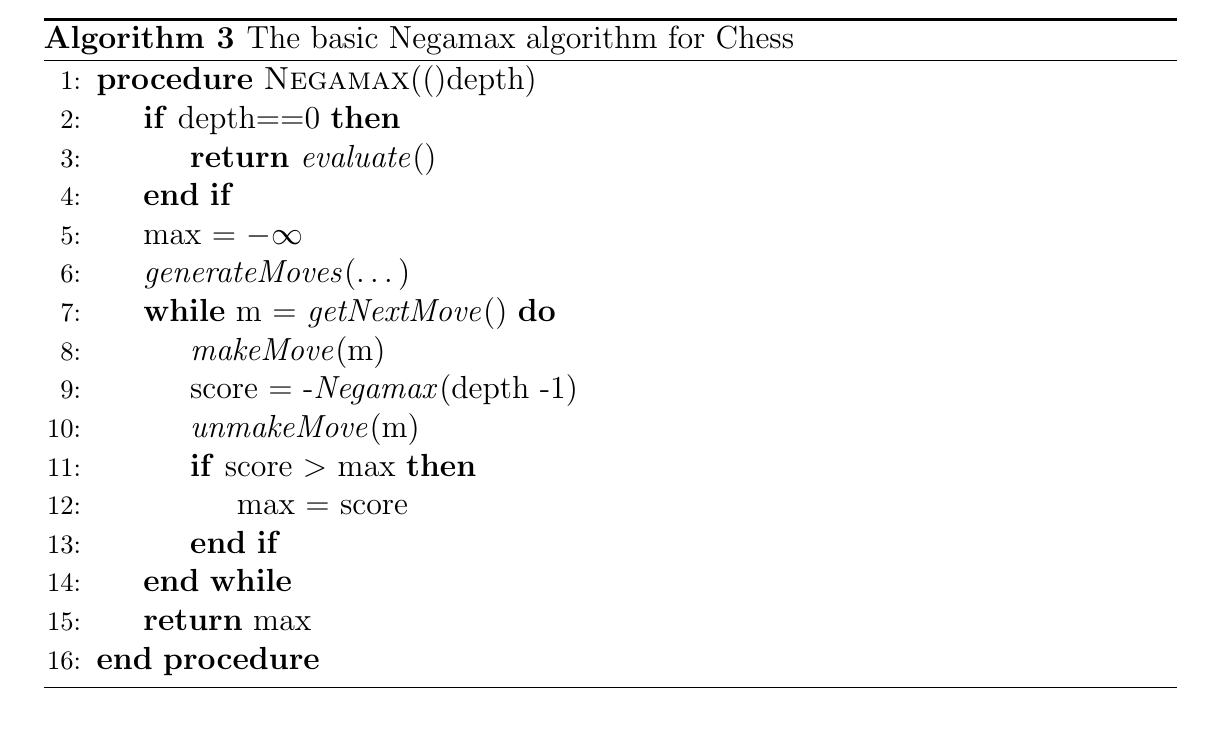
\includegraphics[width=0.8\textwidth]{../img/negamax.png}

\end{frame}

\begin{frame}{Gameplay}{Results}
\begin{itemize}
 \item Played against Sunfish (Ahle, 2015) implements MTD-f for search
 \item Pruned the search space to k=15 moves for every state
 \item 
\end{itemize}
\begin{table}[width=1.0\textwidth]
\tiny
\centering
\begin{tabular}{@{}llllll@{}}
\toprule
{\bf Method Used} & Games Played & Won & Drawn & Lost & 
Details                      \\ \midrule
Top-Prob          & 73           & 7         & 20          & 46         & 
$10\leq maxn\leq 1000$ \\\\
TopProb-Negamax&19     &3        &4		   & 12           & 
$10\leq maxn\leq 100$ \\\\
Evaluation function ($V_{\gamma=0.7}$)&&&&&\\
with Negamax &   21      & 6  &   4           & 11       &  2 \textless Negamax 
depth \textless 5 \\\\
Evaluation function ($V_{\gamma=0.7}$)&&&&&\\
with Negamax& 25        &  16 & 2             & 7       & Negamax depth=4       
                      \\\\
%                   &              &           &             &            &      
  
%                       \\
%                   &              &           &             &            &      
  
%                       \\
%                   &              &           &             &            &      
  
%                       \\ 
                      \bottomrule
\end{tabular}
\caption[Results against negamax]{The table shows the result statistics for 
evaluation of gameplay against sunfish. 
In most of our experiments we limit the 
number of nodes explored by 
Sunfish between 10 to 1000 (chosen randomly on a log scale). For other 
deviations, the details are mentioned in the details column}
\end{table}
\end{frame}

\section{Conclusions}
\begin{frame}{Conclusion}
 \begin{itemize}
  \item We need to evaluate the game play to get an ELO rating for our system.
  \item A possible improvement could be to use a bigram or a trigram input to train the networks. This will help the networks learn the long term tactics.
  \item A faster implementation could be provided by not relying on another chess playing engine to generate search trees.
 \end{itemize}

\end{frame}



{\aauwavesbg
\begin{frame}[plain,noframenumbering]
  \finalpage{Thank you \vspace{1 cm} \\ Questions?}
\end{frame}}
%%%%%%%%%%%%%%%%

\end{document}
